% Template for PLoS
% Version 3.6 Aug 2022
%
% % % % % % % % % % % % % % % % % % % % % %
%
% -- IMPORTANT NOTE
%
% This template contains comments intended 
% to minimize problems and delays during our production 
% process. Please follow the template instructions
% whenever possible.
%
% % % % % % % % % % % % % % % % % % % % % % % 
%
% Once your paper is accepted for publication, 
% PLEASE REMOVE ALL TRACKED CHANGES in this file 
% and leave only the final text of your manuscript. 
% PLOS recommends the use of latexdiff to track changes during review, as this will help to maintain a clean tex file.
% Visit https://www.ctan.org/pkg/latexdiff?lang=en for info or contact us at latex@plos.org.
%
%
% There are no restrictions on package use within the LaTeX files except that no packages listed in the template may be deleted.
%
% Please do not include colors or graphics in the text.
%
% The manuscript LaTeX source should be contained within a single file (do not use \input, \externaldocument, or similar commands).
%
% % % % % % % % % % % % % % % % % % % % % % %
%
% -- FIGURES AND TABLES
%
% Please include tables/figure captions directly after the paragraph where they are first cited in the text.
%
% DO NOT INCLUDE GRAPHICS IN YOUR MANUSCRIPT
% - Figures should be uploaded separately from your manuscript file. 
% - Figures generated using LaTeX should be extracted and removed from the PDF before submission. 
% - Figures containing multiple panels/subfigures must be combined into one image file before submission.
% For figure citations, please use "Fig" instead of "Figure".
% See http://journals.plos.org/plosone/s/figures for PLOS figure guidelines.
%
% Tables should be cell-based and may not contain:
% - spacing/line breaks within cells to alter layout or alignment
% - do not nest tabular environments (no tabular environments within tabular environments)
% - no graphics or colored text (cell background color/shading OK)
% See http://journals.plos.org/plosone/s/tables for table guidelines.
%
% For tables that exceed the width of the text column, use the adjustwidth environment as illustrated in the example table in text below.
%
% % % % % % % % % % % % % % % % % % % % % % % %
%
% -- EQUATIONS, MATH SYMBOLS, SUBSCRIPTS, AND SUPERSCRIPTS
%
% IMPORTANT
% Below are a few tips to help format your equations and other special characters according to our specifications. For more tips to help reduce the possibility of formatting errors during conversion, please see our LaTeX guidelines at http://journals.plos.org/plosone/s/latex
%
% For inline equations, please be sure to include all portions of an equation in the math environment.  For example, x$^2$ is incorrect; this should be formatted as $x^2$ (or $\mathrm{x}^2$ if the romanized font is desired).
%
% Do not include text that is not math in the math environment. For example, CO2 should be written as CO\textsubscript{2} instead of CO$_2$.
%
% Please add line breaks to long display equations when possible in order to fit size of the column. 
%
% For inline equations, please do not include punctuation (commas, etc) within the math environment unless this is part of the equation.
%
% When adding superscript or subscripts outside of brackets/braces, please group using {}.  For example, change "[U(D,E,\gamma)]^2" to "{[U(D,E,\gamma)]}^2". 
%
% Do not use \cal for caligraphic font.  Instead, use \mathcal{}
%
% % % % % % % % % % % % % % % % % % % % % % % % 
%
% Please contact latex@plos.org with any questions.
%
% % % % % % % % % % % % % % % % % % % % % % % %

\documentclass[10pt,letterpaper]{article}
\usepackage[top=0.85in,left=2.75in,footskip=0.75in]{geometry}

% amsmath and amssymb packages, useful for mathematical formulas and symbols
\usepackage{amsmath,amssymb}
\usepackage{newunicodechar}
\newunicodechar{Δ}{\Delta}
\DeclareUnicodeCharacter{03B2}{\textbeta}
\newunicodechar{₂}{$_2$}
\newunicodechar{ }{~}
\newunicodechar{ }{\,}

% Use adjustwidth environment to exceed column width (see example table in text)
\usepackage{changepage}

% textcomp package and marvosym package for additional characters
\usepackage{textcomp,marvosym}

% cite package, to clean up citations in the main text. Do not remove.
\usepackage{natbib} % for \citep and \citet
% \usepackage{cite} % comment out or remove if using natbib

% Use nameref to cite supporting information files (see Supporting Information section for more info)
\usepackage{nameref,hyperref}

% line numbers
\usepackage[right]{lineno}

% ligatures disabled
\usepackage[nopatch=eqnum]{microtype}
\DisableLigatures[f]{encoding = *, family = * }

% color can be used to apply background shading to table cells only
\usepackage[table]{xcolor}
\usepackage{enumitem}
\usepackage{booktabs}

% array package and thick rules for tables
\usepackage{array}

% create "+" rule type for thick vertical lines
\newcolumntype{+}{!{\vrule width 2pt}}

% create \thickcline for thick horizontal lines of variable length
\newlength\savedwidth
\newcommand\thickcline[1]{%
  \noalign{\global\savedwidth\arrayrulewidth\global\arrayrulewidth 2pt}%
  \cline{#1}%
  \noalign{\vskip\arrayrulewidth}%
  \noalign{\global\arrayrulewidth\savedwidth}%
}

% \thickhline command for thick horizontal lines that span the table
\newcommand\thickhline{\noalign{\global\savedwidth\arrayrulewidth\global\arrayrulewidth 2pt}%
\hline
\noalign{\global\arrayrulewidth\savedwidth}}


% This is for Supplementary
\usepackage{graphicx}      % already in almost every template
\usepackage{subcaption}    % gives sub-figures + \subref
\usepackage{placeins}      % lets us slam a barrier before the SI
\usepackage[margin=1in]{geometry}



% ---------- helper to switch counters to S-numbers ----------
\newcommand{\beginsupplement}{%
  \setcounter{table}{0}%
  \renewcommand{\thetable}{S\arabic{table}}%
  \setcounter{figure}{0}%
  \renewcommand{\thefigure}{S\arabic{figure}}}

% 2) Define a macro \beginsupplement that:
%    • Resets the figure/table counters
%    • Prefixes future figures/tables with “S”
\usepackage{etoolbox} % for \pretocmd and \setcounter


% Remove comment for double spacing
%\usepackage{setspace} 
%\doublespacing

% Text layout
\raggedright
\setlength{\parindent}{0.5cm}
\textwidth 5.25in 
\textheight 8.75in

% Bold the 'Figure #' in the caption and separate it from the title/caption with a period
% Captions will be left justified
\usepackage[aboveskip=1pt,labelfont=bf,labelsep=period,justification=raggedright,singlelinecheck=off]{caption}
\renewcommand{\figurename}{Fig}

% Use the PLoS provided BiBTeX style


% Remove brackets from numbering in List of References
\makeatletter
\renewcommand{\@biblabel}[1]{\quad#1.}
\makeatother

% links
\usepackage{hyperref}


% Header and Footer with logo
\usepackage{lastpage,fancyhdr,graphicx}
\usepackage{epstopdf}
%\pagestyle{myheadings}
\pagestyle{fancy}
\fancyhf{}
%\setlength{\headheight}{27.023pt}
%\lhead{\includegraphics[width=2.0in]{PLOS-submission.eps}}
\rfoot{\thepage/\pageref{LastPage}}
\renewcommand{\headrulewidth}{0pt}
\renewcommand{\footrule}{\hrule height 2pt \vspace{2mm}}
\fancyheadoffset[L]{2.25in}
\fancyfootoffset[L]{2.25in}
\lfoot{\today}

%% Include all macros below

\newcommand{\lorem}{{\bf LOREM}}
\newcommand{\ipsum}{{\bf IPSUM}}



%% END MACROS SECTION
\usepackage{graphicx}
\usepackage[aboveskip=1pt,labelfont=bf,labelsep=period,justification=raggedright,singlelinecheck=off]{caption}
\usepackage{placeins}

\begin{document}
\vspace*{0.2in}

% Title must be 250 characters or less.
\begin{flushleft}
{\Large
\textbf\newline{Sorghum Lipidomics Database} % Please use "sentence case" for title and headings (capitalize only the first word in a title (or heading), the first word in a subtitle (or subheading), and any proper nouns).
}
\newline
% Insert author names, affiliations and corresponding author email (do not include titles, positions, or degrees).
\\
Nirwan Tandukar\textsuperscript{1,2\Yinyang},
Ruthie Stokes\textsuperscript{3},
Name4 Surname\textsuperscript{2},
Name5 Surname\textsuperscript{2\ddag},
Name6 Surname\textsuperscript{2\ddag},
Rubén Rellán Álvarez\textsuperscript{1,3*},

\bigskip
\textbf{1} Department of Genetics and Genomics, North Carolina State University, Raleigh, NC, USA
\\
\textbf{2} Department of Bioinformatics, North Carolina State University, Raleigh, NC, USA
\\
\textbf{3} Department of Molecular and Structural Biochemistry,  North Carolina State University, Raleigh, NC, USA
\\
\bigskip


% Insert additional author notes using the symbols described below. Insert symbol callouts after author names as necessary.
% 
% Remove or comment out the author notes below if they aren't used.
%
% Primary Equal Contribution Note
\Yinyang These authors contributed equally to this work.

% Additional Equal Contribution Note
% Also use this double-dagger symbol for special authorship notes, such as senior authorship.
\ddag These authors also contributed equally to this work.

% Current address notes
\textcurrency Current Address: Dept/Program/Center, Institution Name, City, State, Country % change symbol to "\textcurrency a" if more than one current address note
% \textcurrency b Insert second current address 
% \textcurrency c Insert third current address

% Deceased author note
\dag Deceased

% Group/Consortium Author Note
\textpilcrow Membership list can be found in the Acknowledgments section.

% Use the asterisk to denote corresponding authorship and provide email address in note below.
* correspondingauthor@institute.edu

\end{flushleft}
% Please keep the abstract below 300 words
\section*{Abstract}
SAP lines



\linenumbers

% Use "Eq" instead of "Equation" for equation citations.
\section*{Introduction}

\subsection*{Lipid remodelling under abiotic constraints}

Plants remodel their membranes in a highly‐orchestrated manner when temperature or nutrient supply is sub‑optimal.  Below we summarise the characteristic fingerprints for \textbf{cold}, \textbf{phosphorus} and \textbf{nitrogen} stress, with emphasis on (i) class ratios that can be used as diagnostic indicators and (ii) individual molecular species that act as markers in lipidomic data sets.

%--------------------------------------------------------------------
\subsubsection*{Cold stress}
\label{sec:cold}

\begin{enumerate}[label=\textbf{\arabic*.}, leftmargin=1.2em]
  \item \textbf{Higher acyl‑chain unsaturation.}  Cold‐tolerant genotypes accumulate poly‑unsaturated fatty acids—principally 18\,:3, 18\,:2 and 18\,:1—leading to a higher double‑bond index (DBI) and preventing membrane rigidification at low temperature \citep[pp.~431–440, 460]{Low_temp_stress_Bhattacharya}.  An increase in DBI is consistently reported in tolerant lines of \textit{Arabidopsis}, maize and peanut \citep[pp.~11–12]{Lipid_transcriptome_Cold_stress_Yu}.

  \item \textbf{Class‑level reshaping.}  
        \begin{itemize}
          \item Poly‑unsaturated PC, PE, PG, MGDG and DGDG species rise, whereas their saturated counterparts decline \citep[pp.~3–4]{Low_temperatures_Wang,Low_temp_stress_Bhattacharya}.  
          \item The bilayer/non‑bilayer ratio, \(\mathrm{(PC+DGDG)/(PE+MGDG)}\), increases, stabilising the lamellar phase of membranes during freezing events \citep[pp.~492–493]{Low_temp_stress_Bhattacharya}.  
          \item Phosphatidic acid (PA) and lysophospholipids (LPC, LPE) surge, reflecting activation of phospholipase D and A, respectively \citep[pp.~456, 472--474]{Low_temp_stress_Bhattacharya}.
        \end{itemize}

  \item \textbf{Species‑level markers.}  In maize, PA\,36:5, PA\,36:6, DAG\,36:5 and DAG\,36:6 are elevated, whereas MGDG\,36:5 and multiple PC species decline \citep[pp.~6–8]{cold_tolerance_maize_Shi}.  Tolerant cultivars show higher TAG and lower DAG/TAG ratios compared with sensitive lines \citep[pp.~11]{Lipid_transcriptome_Cold_stress_Yu}.

  \item \textbf{Lipid signalling.}  PLD- and PLA‑derived PA and lyso‑lipids act as second messengers, triggering cold‐responsive gene networks \citep[pp.~454–456]{Low_temp_stress_Bhattacharya}.

  \item \textbf{Functional outcome.}  Increased unsaturation and altered bilayer propensity maintain a fluid–crystalline phase, securing electron transport and nutrient transport across membranes at low temperature \citep[pp.~463–465]{Low_temp_stress_Bhattacharya}.
\end{enumerate}

%--------------------------------------------------------------------
\subsubsection*{Phosphorus deprivation}
\label{sec:phosphorus}

\begin{enumerate}[label=\textbf{\arabic*.}, leftmargin=1.2em]
  \item \textbf{Phospholipid depletion.}  Major phospholipids (PC, PE, PG, PI, PS, PA) decline sharply as they serve as an internal Pi source; in soybean leaves every phospholipid class decreased under Pi limitation \citep[pp.~1,\,3,\,5]{lipid_remodeling_low_P_Saito}.

  \item \textbf{Compensatory rise of non‑P lipids.}  MGDG, DGDG, SQDG and the diagnostic glucuronosyldiacylglycerol (GlcADG) accumulate to preserve membrane surface area \citep[pp.~3--4]{Phosphate_deficiency_Wang}.  GlcADG can increase up to 14‑fold in soybean \citep{lipid_remodeling_low_P_Saito}.

  \item \textbf{Diagnostic ratio.}  The phospholipid/galactolipid ratio (PL/GL) drops from \(\sim\)0.3 (P‐sufficient) to \(\le 0.05\) under severe P stress in field‐grown camelina \citep[page~4]{Phosphate_deficiency_Wang}.

  \item \textbf{Tissue specificity.}  Older leaves are remodelled first, exporting Pi to developing tissues \citep[pp.~1,\,5]{lipid_remodeling_low_P_Saito}.

  \item \textbf{Enzymatic drivers.}  Phospholipase C/D hydrolyse PC and PE; MGDG/DGDG and SQDG synthases are up‑regulated to supply the replacement lipids \citep[pp.~1–2, 6]{Phosphate_scaracity_Xue}.
\end{enumerate}

%--------------------------------------------------------------------
\subsubsection*{Nitrogen deprivation}
\label{sec:nitrogen}

\begin{enumerate}[label=\textbf{\arabic*.}, leftmargin=1.2em]
  \item \textbf{Chloroplast glycolipids.}  Rapeseed shows an 18 % (leaf) to 35 % (root) reduction in MGDG; DGDG declines by 23 % in roots, resulting in a suppressed \(\mathrm{MGDG/DGDG}\) ratio \citep[pp.~5--9]{nitrogen_deficiency_lipid_Yang}.

  \item \textbf{Phospholipid curtailment.}  PC, PE, PI, PS and PA all decrease markedly, the latter by more than 90 % in both organs \citep{nitrogen_deficiency_lipid_Yang}.

  \item \textbf{Storage lipids.}  TAG remains unchanged in rapeseed but accumulates in mature tea leaves under low N, suggesting carbon re‑allocation from photosynthetic (N‑rich) to storage pools \citep[pp.~6--7]{Nitrogen_fertilizer_Ruan}.

  \item \textbf{Integrated carbon‑nitrogen balance.}  Lower nitrogen leaves a surplus of assimilated carbon; plants divert it into TAG or into highly unsaturated MGDG 36:5/36:6 species observed in tea shoots at high N \citep{Nitrogen_fertilizer_Ruan}.
\end{enumerate}

%--------------------------------------------------------------------
\subsubsection*{Synthesis}

Cold, P and N stress each trigger a distinctive yet overlapping pattern of lipid remodelling:

\begin{itemize}
  \item \textbf{Cold} prioritises \emph{unsaturation} and bilayer‑to‑non‑bilayer balance to maintain fluidity.  
  \item \textbf{Pi starvation} reallocates phosphorus by replacing phospho‑lipids with galacto‑ and sulfo‑lipids, sharply lowering the PL/GL ratio.  
  \item \textbf{N starvation} down‑regulates chloroplast glycolipids and phospholipids, sometimes storing excess carbon as TAG.  
\end{itemize}

These shifts are mirrored in our sorghum data: unsaturation indices rise under early low‑temperature planting; the \(\mathrm{DGDG/MGDG}\) and \(\mathrm{SQDG/PG}\) ratios increase under P‑limited, low‑input conditions; and TAG/PC as well as \(\mathrm{TG/DG}\) ratios escalate when available nitrogen is low (see Sections \ref{sec:cold}, \ref{sec:phosphorus} and \ref{sec:nitrogen}).

- Stress in plants specifically in sorghum

- Cold stress

- low Nitrogen

- low Phosphorus

- Relate to climate change?



%---------------------------------------------------------------
\begin{table}[ht]
\centering
\small
\setlength{\tabcolsep}{6pt}
\renewcommand{\arraystretch}{1.15}
\begin{tabular}{@{}p{2.3cm} p{4.2cm} p{1.3cm} p{4.5cm} p{1.7cm}@{}}
\toprule
\textbf{Stress} & \textbf{Key lipid class / molecular species} & \textbf{Direction\textsuperscript{a}} & \textbf{Diagnostic (ratio) or remark} & \textbf{Ref.} \\
\midrule
\multirow{6}{*}{\textbf{Cold}} 
 & Poly‑unsaturated FA (18:3, 18:2, 18:1)            & $\uparrow$ & Higher double‑bond index (DBI)                                & \citet{Low_temp_stress_Bhattacharya} \\
 & Unsat.\ PC, PE, PG, MGDG, DGDG                     & $\uparrow$ & Bilayer lipids enriched                                        & \citet{Low_temperatures_Wang}        \\
 & PA (incl.\ PA\,36:5;\,36:6)                        & $\uparrow$ & PLD activation; signalling                                     & \citet{cold_tolerance_maize_Shi}     \\
 & LPC, LPE                                           & $\uparrow$ & PLA activity                                                   & \citet{Low_temp_stress_Bhattacharya} \\
 & DAG\,36:5;\,36:6                                   & $\uparrow$ & Mobilisation of PC unsat.\ chains                             & \citet{cold_tolerance_maize_Shi}     \\
 & TAG (total)                                        & $\uparrow$ & \textit{cf.}\ DAG/TAG $\downarrow$ in tolerant lines           & \citet{Lipid_transcriptome_Cold_stress_Yu} \\
 \cmidrule{2-5}
 & \multicolumn{2}{@{}l}{\textit{Cold ratios}}       & (PC\,+\,DGDG)/(PE\,+\,MGDG)\:$\uparrow$; \ DAG/TAG\:$\downarrow$ & \citet{Low_temp_stress_Bhattacharya} \\
\midrule
\multirow{5}{*}{\textbf{P deficiency}} 
 & PC, PE, PG, PI, PS, PA                             & $\downarrow$ & Release of Pi pool                                            & \citet{lipid_remodeling_low_P_Saito} \\
 & MGDG, DGDG                                          & $\uparrow$  & Galacto‑lipid replacement                                     & \citet{Phosphate_deficiency_Wang}    \\
 & SQDG                                               & $\uparrow$  & Sulfo‑lipid substitution                                      & \citet{Phosphate_deficiency_Wang}    \\
 & GlcADG                                             & $\uparrow$  & Pi‑stress biomarker (14‑fold)                                 & \citet{lipid_remodeling_low_P_Saito} \\
 & \multicolumn{2}{@{}l}{\textit{P ratios}}           & PL/GL $\downarrow$ (to $\le$ 0.05); DGDG/MGDG $\uparrow$        & \citet{Phosphate_deficiency_Wang}    \\
\midrule
\multirow{5}{*}{\textbf{N deficiency}} 
 & MGDG (leaf, root)                                  & $\downarrow$ & 18–35 \% reduction                                            & \citet{nitrogen_deficiency_lipid_Yang} \\
 & DGDG (root)                                        & $\downarrow$ & 24 \% reduction                                               & \citet{nitrogen_deficiency_lipid_Yang} \\
 & PC, PE, PI, PS, PA                                 & $\downarrow$ & PA $\downarrow$ > 90 \%                                       & \citet{nitrogen_deficiency_lipid_Yang} \\
 & TAG (mature tea leaves)                            & $\uparrow$  & Carbon sink under low N                                       & \citet{Nitrogen_fertilizer_Ruan}      \\
 & \multicolumn{2}{@{}l}{\textit{N ratios}}           & MGDG/DGDG $\downarrow$; TAG/PC $\uparrow$; TG/DG $\uparrow$     & \citet{nitrogen_deficiency_lipid_Yang} \\
\bottomrule
\multicolumn{5}{l}{\footnotesize \textsuperscript{a}\,$\uparrow$ increase, $\downarrow$ decrease relative to control or sufficient nutrient.}
\end{tabular}
\caption{Core lipid markers and class ratios characterising cold, phosphorus and nitrogen stress as distilled from the literature survey.  Arrows indicate the direction of change in stressed tissues.}
\label{tab:lipid_markers}
\end{table}
%---------------------------------------------------------------


\subsection*{OPLS-DA}
4. Supervised multivariate discrimination of the lipidomes
4.1 What OPLS‑DA does—in plain language
Orthogonal‑Projection to Latent Structures Discriminant Analysis (OPLS‑DA) is a supervised extension of Principal‑Component Analysis that forces the first latent component to explain only variance that is correlated with a user‑defined class vector (here, Control vs Low‑input). Any systematic variation that is orthogonal to class membership—batch differences, genotype heterogeneity, stochastic noise—is captured in subsequent, “orthogonal” components.
The outcome is a model that

separates classes as strongly as possible along a single predictive axis (t1),

isolates uninformative variance on orthogonal axes (to1, to2, …), and

provides a Variable‑Importance in Projection (VIP) score for every lipid, ranking its contribution to class separation.

Because the method is supervised, we rigorously guard against over‑fitting by (i) k‑fold cross‑validation (Q²) and (ii) permutation testing.

4.2 Model quality and diagnostic overview (Fig. 6a–d)
<div align="center"><em>Insert composite “overview” panel here</em></div>
Panel (a) – Component summary 
The model contains one predictive component (p1) and two orthogonal components (o1, o2). Predictive component p1 alone explains 94 % of the class variance (R²Y) and 94 % of its cross‑validated predictability (Q²Y), well above the commonly accepted 0.5 threshold (grey reference line). Orthogonal components capture residual variation in the lipid matrix (R²X ≈ 0.70 in total) that is unrelated to treatment.

Panel (b) – Permutation test 
Two‑hundred random permutations of the class vector were fitted to the same data (grey dots). None of the permuted models approaches the real model’s Q² or R² (black bars on the right). The probability of obtaining an equal or better model by chance is pR²Y = 0.05; pQ² = 0.05, confirming that the discrimination is not an over‑fit artefact.

Panel (c) – Observation diagnostics 
Score‑distance (SD, leverage) is plotted against orthogonal distance (OD, residual variance). Dashed lines denote the 95 % Hotelling T² limits. Only five genotypes (labels s441, s736, s447…) exceed one or both thresholds; visual inspection of chromatograms revealed no technical issue, hence they were retained.

Panel (d) – Score plot 
Each point represents a genotype; blue = Control, red = Low‑input. The two classes form well‑separated, compact clouds along the predictive axis t1 (39 % of total lipid variance), while the orthogonal axis to1 (30 %) captures within‑class dispersion. The 95 % confidence ellipse encloses every sample except the mild outliers identified in panel (c). Together with the high Q², this demonstrates a robust lipidomic signature of the Low‑input treatment.

4.3 Discriminatory lipids revealed by VIP analysis (Fig. 6e)
<div align="center"><em>Insert VIP bar plot (top 30) here</em></div>
VIP values quantify how strongly each lipid contributes to the predictive component. A conservative cut‑off of VIP > 1.3 (dashed line) yielded 28 discriminatory species (Supplementary Table S7). The top ten are displayed in Fig. 6e and encompass several structural classes:

Rank	Lipid (annotation)	Class	VIP	Change in Low‑input†
1	Nostoxanthin	Terpenoid	1.88	 ↑ 4.1‑fold
2	Triethylene‑glycol bis(2‑ethyl‑hexanoate)	Plasticizer ‡	1.82	 ↓ 3.6‑fold
3	ε‑Decalactone	Organic compound	1.79	 ↑ 2.9‑fold
…	…	…	…	…

† Fold‑change refers to median linear intensity.
‡ Likely exogenous contaminant; retained for completeness but excluded from biological discussion.

Biologically meaningful drivers include:

Triacyl‑glycerols TG(56:6), TG(46:0) – consistently enriched under Low‑input, supporting the nitrogen‑remobilisation hypothesis (Fig. 6e, pale‑blue bars).

Phosphatidylethanolamine PE(34:1) – depleted in Low‑input, aligning with the phospholipid‑to‑glycolipid replacement model under combined low P/low N.

β‑Sitosterol – a sterol known to modulate membrane order, markedly increased (VIP 1.55), coherent with the observed membrane‑integrity ratios (Fig. 5).

These VIP‑identified species therefore corroborate and extend the univariate ratio analysis.

4.4 Interpretation
The OPLS‑DA model demonstrates that field Low‑input treatment imprints a strong, coherent lipidomic signature across 350–380 sorghum genotypes, explaining > 80 % of class variance with excellent predictability.

Discriminating lipids belong to storage (TG), membrane (PE) and signalling (sterols, terpenoids) pools, suggesting a coordinated adjustment of carbon and nutrient allocation.

The very limited number of statistical outliers and the stringent permutation validation underline the robustness of the result.

Together, these findings establish a quantitative link between agronomic low‑input management and the sorghum lipidome, and highlight specific lipid species that can serve as biomarkers for future breeding or physiological studies.

\section*{Materials and methods}

\subsection*{Plant material and growth conditions}
Our study used the Sorghum Association Panel (SAP), a 400‑accession diversity panel assembled to capture a wide range of genetic and phenotypic variation. The collection comprises temperate‑adapted breeding lines alongside tropical landraces. Accessions span the five recognized botanical races, bicolor, caudatum, durra, guinea, and kafir, which together reflect multiple domestication and post‑domestication adaptation events.

 SAP was initially genotyped with simple sequence repeat markers and later with low-coverage genotyping by sequencing (GBS). To obtain a more complete variant collection, Boatwright et al. resequenced all entries by whole genome sequencing (WGS) to a mean depth of 38× (range 25–72×). The variant based on the WGS data yielded approximately 43.98M polymorphisms, comprising ~38M SNPs, ~5M short insertions/deletions, and ~17×10\^5 copy‑number variants. Approximately 50\% of the 5 kb genomic windows contained variants detectable only in the WGS data set, underscoring the markedly higher genomic coverage of WGS compared to GBS. Whereas the GBS variants were heavily biased toward genic regions, the WGS calls were distributed more evenly between the genic and intergenic sequences.

The population structure analysis partitioned the panel into six genetic groups that mirrored the botanical races and the main breeding groups. Genome‑wide linkage disequilibrium decayed to half‑maximum within ~20 kb, with chromosome‑specific departures from this average. The resulting high‑density variant map and well‑characterised structure make the resequenced SAP a powerful resource for diversity and whole genome wide association studies (GWAS).


We evaluated SAP accessions under two distinct field conditions over two growing seasons (2019 and 2020) at Pee Dee Research and Education Center in Clemson University, Florence, South Carolina. Standard agronomic inputs with adequate nitrogen (N) and phosphorus (P) and a normal planting date, which we define as a "control". Low availability of N and P, combined with early planting to simulate cooler and more stressful environments, which we define as "low input". Fig~\ref{fig1}


\subsection*{Lipid extraction and analysis}


\subsection*{Lipidomics data processing}
First, the raw peak intensity signals were filtered to remove any feature with a retention time below 1 min. The intensity columns at the sample level were then isolated and each was renamed by extracting the run number and the “PI” label from the original LC-MS filenames. The columns were sorted in ascending run order so that the downstream matrices reflect the chronological injection sequence.

Next, blank filtering was applied by calculating, for each feature, the minimum signal across all biological samples and the mean signal in the set of blank injections. Features whose minimal sample value was less than 10× the blank average were removed. Then, all blank and check injections were removed, leaving only genuine sample peaks which were used for further analysis.

For quality control, the remaining injections of “QC” were pulled from the filtered table and explored using summary statistics and box plots (should i do these as well ????? PCA, heat maps, and correlation matrices) to verify signal consistency between batches (Supplementary Fig. 1). Any features or runs that showed obvious outlier behavior in these diagnostics were flagged for removal from subsequent analyses.

The cleaned data were then prepared for SERRF normalization (Systematic Error Removal Using Random Forest) (ref): sample and QC labels were added as the first two rows, followed by run numbers and batch identifiers derived from an external batch-run mapping file. The resulting CSV was uploaded to the SERRF server (https://slfan2013.github.io/SERRF-online/#), and the normalized output was retrieved.

Post-SERRF, only biological samples were retained. Lipid features with more than 50 \% zero values were dropped, and remaining zeros were replaced by two-thirds of the lowest nonzero value per feature to avoid potential infinite log transformations.


\subsection*{Lipid annotation}

\subsection*{Lipid quantification and normalization.}

The raw peak intensities were summed by traditional lipid classes (Supplementary Table 1) for each sample. To control for run-to-run variation, we divided each class sum by the total intensity across all classes in that sample and reported it as a percentage of total ion current (TIC). The percentages of the mean classes were calculated separately for the control groups (n = 384) and the low input group (n = 362) and displayed as bar charts stacked with 100 \%. For each of the classes, we also summarized their subclasses. For example, for the Terpenoid subclasses, we summarized each individual species (e.g., Lycopene, β-Carotene, α-Tocopherol), calculated its fraction of the sum of Terpenoid within each sample, and then averaged those percentages by condition. The composition of the species level was also visualized as stacked paired bars 100 \% (control vs. low input) alongside a small table of mean percentages with matching color swatches. We also calculated per-sample ratios for important stress responses.

\subsection*{Statistical analysis}

\subsection*{Genome-wide association analysis}  
Genome-wide association studies were conducted separately for each lipid trait and for each field condition using the mixed linear model (MLM) implemented in GEMMA (v2.3) (ref).  A centered relatedness matrix (kinship) was estimated from the SNP genotype data to control for population structure and cryptic relatedness.  For each individual lipid, we fitted the MLM with the kinship matrix to account for population stratification.  In addition to single-trait scans, lipids were grouped by biochemical class (see Supplementary Table 1), and a PCA was performed within each class to capture the major axes of variation; we then ran separate GWAS on the first two PCs specific to the class.  All association tests produced *p * values, which were adjusted for multiple comparisons using the Benjamini-Hochberg false discovery rate (FDR), with FDR < 0.05 considered significant.

\subsection*{Candidate gene annotation}  
All the SNPs were mapped to the Sorghum bicolor reference genome v3.1 (BTx623).  For each marker, we defined a 50 kb interval (25 kb upstream and downstream) and extracted all gene models within that window.  Functional annotations and homology information were retrieved from Phytozome (https://phytozome.jgi.doe.gov), SorghumBase (https://sorghumbase.com), and TAIR (for Arabidopsis thaliana orthologs).  The annotated genes were manually selected for their known roles in the N, P, or cold response, or lipid metabolism.  Finally, we tabulated the recurrence of each candidate gene in all lipid GWAS results and summarized the most frequent genes based on -log10(p-values) >= 7 or 5.

\subsection*{Hierarchical clustering}
For each lipid and genotypes, we performed a hierarchical clustering using the \texttt{hclust} function in R.  Before clustering, the lipid intensities were scaled to zero mean and unit variance.  A Euclidean distance matrix was calculated and the groups were merged according to Ward's minimum variance criterion (Ward.D2).  The dendrograms were rendered with the \texttt{dendextend} package, and two-dimensional clustergrams were generated using the \texttt{ clustergram.R} script.  

\subsection*{Dimensionality reduction (PCA, UMAP, t-SNE)}  
To identify common patterns based on lipids and genotypes, we performed three-dimensionality reduction techniques in R: principal component analysis (PCA), uniform manifold approximation and projection (UMAP), and stochastic neighbor embedding distributed by t (t-SNE).  Before all analyzes, each data matrix (lipids or genotypes) was centered and scaled so that each variable contributes equally to the distance calculations.

For PCA, we used the \texttt{prcomp()} function in base R, retaining the first two principal components for visualization.  Scree plots and loading vectors were examined to identify which lipids or variants drive the greatest variance.  

For nonlinear embedding, we employ UMAP via the \texttt{uwot} package (\texttt{umap()} function) with default settings (n\_neighbors = 15, min\_dist = 0.1) to capture both local and global structure.  We also ran t-SNE using the \texttt{Rtsne} package, setting perplexity = 30 (which could be changed) and a maximum of 1,000 iterations.  

The resulting two-dimensional coordinates were plotted with \texttt{ggplot2}, colored by biochemical class.

\subsection*{Pathway enrichment analysis}

\subsection*{Data availability}



% Results and Discussion can be combined.
\section*{Results}

\subsection*{Overview of lipid profiles}

Instrument performance was measured using total ion current (TIC) traces throughout the injection sequence for batches C (Supplementary Fig. \ref{fig:S1A}) and LI (Supplementary Fig. \ref{fig:S1B}). As expected, the blanks (gray) remain near zero TIC, the internal standards (green) cluster tightly around their nominal signal, and the quality controls (red) track reproducibly throughout the run. The injections of samples (blue) exhibit the highest TIC with no isolated outliers or sudden jumps. These profiles confirm that instrument performance was stable over time, with consistent sensitivity and no evidence of progressive signal decay or unexpected artifacts.

In sets C and LI, the relative standard deviation of the sample (RSD) for all lipid characteristics decreased from 3. 86 \% and 1. 18 \% (raw data)  to 0. 94 \% and 0. 51 \%, respectively, after normalization of the SERRF (Supplementary Figs. \ref{fig:S1A} and \ref{fig:S1B}, top panel). This reduction in technical variability demonstrates that SERRF effectively removes batch-related effects, producing more consistent peak areas across injections. Similarly, PCA of the signal pre- and post-SERRF shows that the points cluster tightly, indicating that most of the remaining variance is biological rather than instrumental (Supplementary Figs. \ref{fig:S1A} and \ref{fig:S1B}, bottom panel).


The total number of different lipid species and their classes identified under C and LI conditions is shown in the Supplementary Figure \ref{fig:S3A}, Supplementary Figure \ref{fig:S3B} and  \href{https://docs.google.com/spreadsheets/d/1SB90-QLYheKEzmHCUIh1UfgkrtbL064s8Oo5BfwFaV0/edit?gid=1876149577#gid=1876149577}{Supplementary Table S1A}. In particular, triacylglycerols (TG) exhibit greater species diversity with low input (85 species) compared to Control (74 species), while phosphatidylcholines (PC) decrease from 33 species in C to 26 species in LI. Monoacylglycerols (MG) also decline from 7 species in C to 3 species in LI, while phosphatidylethanolamines (PE) increase slightly (11 species in C versus 12 in LI) (Supplementary Figure \ref{fig:S3B}, \href{https://docs.google.com/spreadsheets/d/1SB90-QLYheKEzmHCUIh1UfgkrtbL064s8Oo5BfwFaV0/edit?gid=1876149577#gid=1876149577}{Supplementary Table 1B}). When aggregated by lipid class (Supplementary Figure \ref{fig:S3C}), glycerolipids increase from 86 classes in Control to 96 in LI, while glycerophospholipids fall from 39 classes in C to 35 in LI, driven primarily by the loss of PC subspecies. The glycoglycerolipids remain essentially unchanged (25 in C, 24 in LI), and small molecule classes such as sphingolipids (SM), lysophospholipids (LPC, LPE), free fatty acids (FA), phosphoglycerols (PG) and ceramides (Cer) each remain at one or two detected species under both conditions, possibly due to the inability of the mass spectrometer to identify those small signals (Supplementary Figures \ref{fig:S3A} and \ref{fig:S3B} and ). A total of 301 (217 in C, 254 in LI) species were detected across both workflows, 47 (15.6\%) are unique to C, 84 (27.9\%) are unique to LI and 170 (56.5\%) are shared (Supplementary Figure \ref{fig:S3C}). Thus, in the LI condition, (1) the diversity of TG increases, (2) the diversity of PC decreases, (3) the diversity of PE slightly increases, and (4) approximately 57\% of the lipid species are common to both datasets, with around 15\% unique to C and 29\% unique to LI.

We also calculated the contribution of each lipid species and class to the total ion current (TIC) in each sample. The percentage of TIC values was averaged in all C (n = 384) and in all LI (n = 362). Any species or class whose mean percentage fell below 3\% in both conditions was not labeled in our visualization. At the species level, PC exhibits the largest depletion under LI handling. PC species collectively account for approximately 13.3\% of TIC in the C samples but drop to approximately 7. 4\% with LI (Fig. \ref{fig:1A_lipid_species}). In contrast, monogalactosyldiacylglycerol (MGDG) species increase from 37.1\% of TIC in C to 39.9\% in LI, making MGDG the single largest relative gain among abundant species. The sulfoquinovosyldiacylglycerol species (SQDG) drop from 8. 2\% to 3. 9\%, and the TG species rise from 5. 1\% to 9. 7\%. Together, these shifts illustrate that mid-abundance glycerolipid species (MGDG and TG) become more dominant when input is limited, while key glycerophospholipids (such as PC) and pigment‐derived lipids (SQDG) are comparatively underrepresented (Fig. \ref{fig:1A_lipid_species}).

When we divided the lipids into broader lipid classes, the same pattern emerged at the class level as well. In C, glycoglycerolipids (MGDG + DGDG) account for approximately 60 4\% of TIC, while under LI, this increases to approximately 65 7\%. In contrast, glycerophospholipids (PC + PE + PG + LPC + LPE) decrease from 13.5\% in C to 8. 5\% in LI, reflecting the loss driven by PC observed at the species level. The most striking class-level depletions are tetrapyrroles (chlorophyll-derived pigments), which drop from 14.5\% to 9.5\% (Fig. \ref{fig:1B_lipid_class}).

In summary, the LI condition marked a redistribution of leaf lipid TIC: the combined glycerolipid pool (MGDG + DGDG + TG) gains approximately 10 percentage points of relative abundance, at the expense of glycerophospholipids (primarily PC) and tetrapyrroles. These results underscore how reduced starting material skews the measured lipidome toward galactolipid-rich membranes (e.g., MGDG / DGDG) and neutral storage lipids (TG), while under‐sampling key phospholipids and pigment‐associated lipids.


\begin{figure}[htp]
  \centering

  %----------------------------------------------------
  %  (A) Top panel: species‐level lipid composition
  %----------------------------------------------------
  \begin{subfigure}[t]{\textwidth}
    \centering
    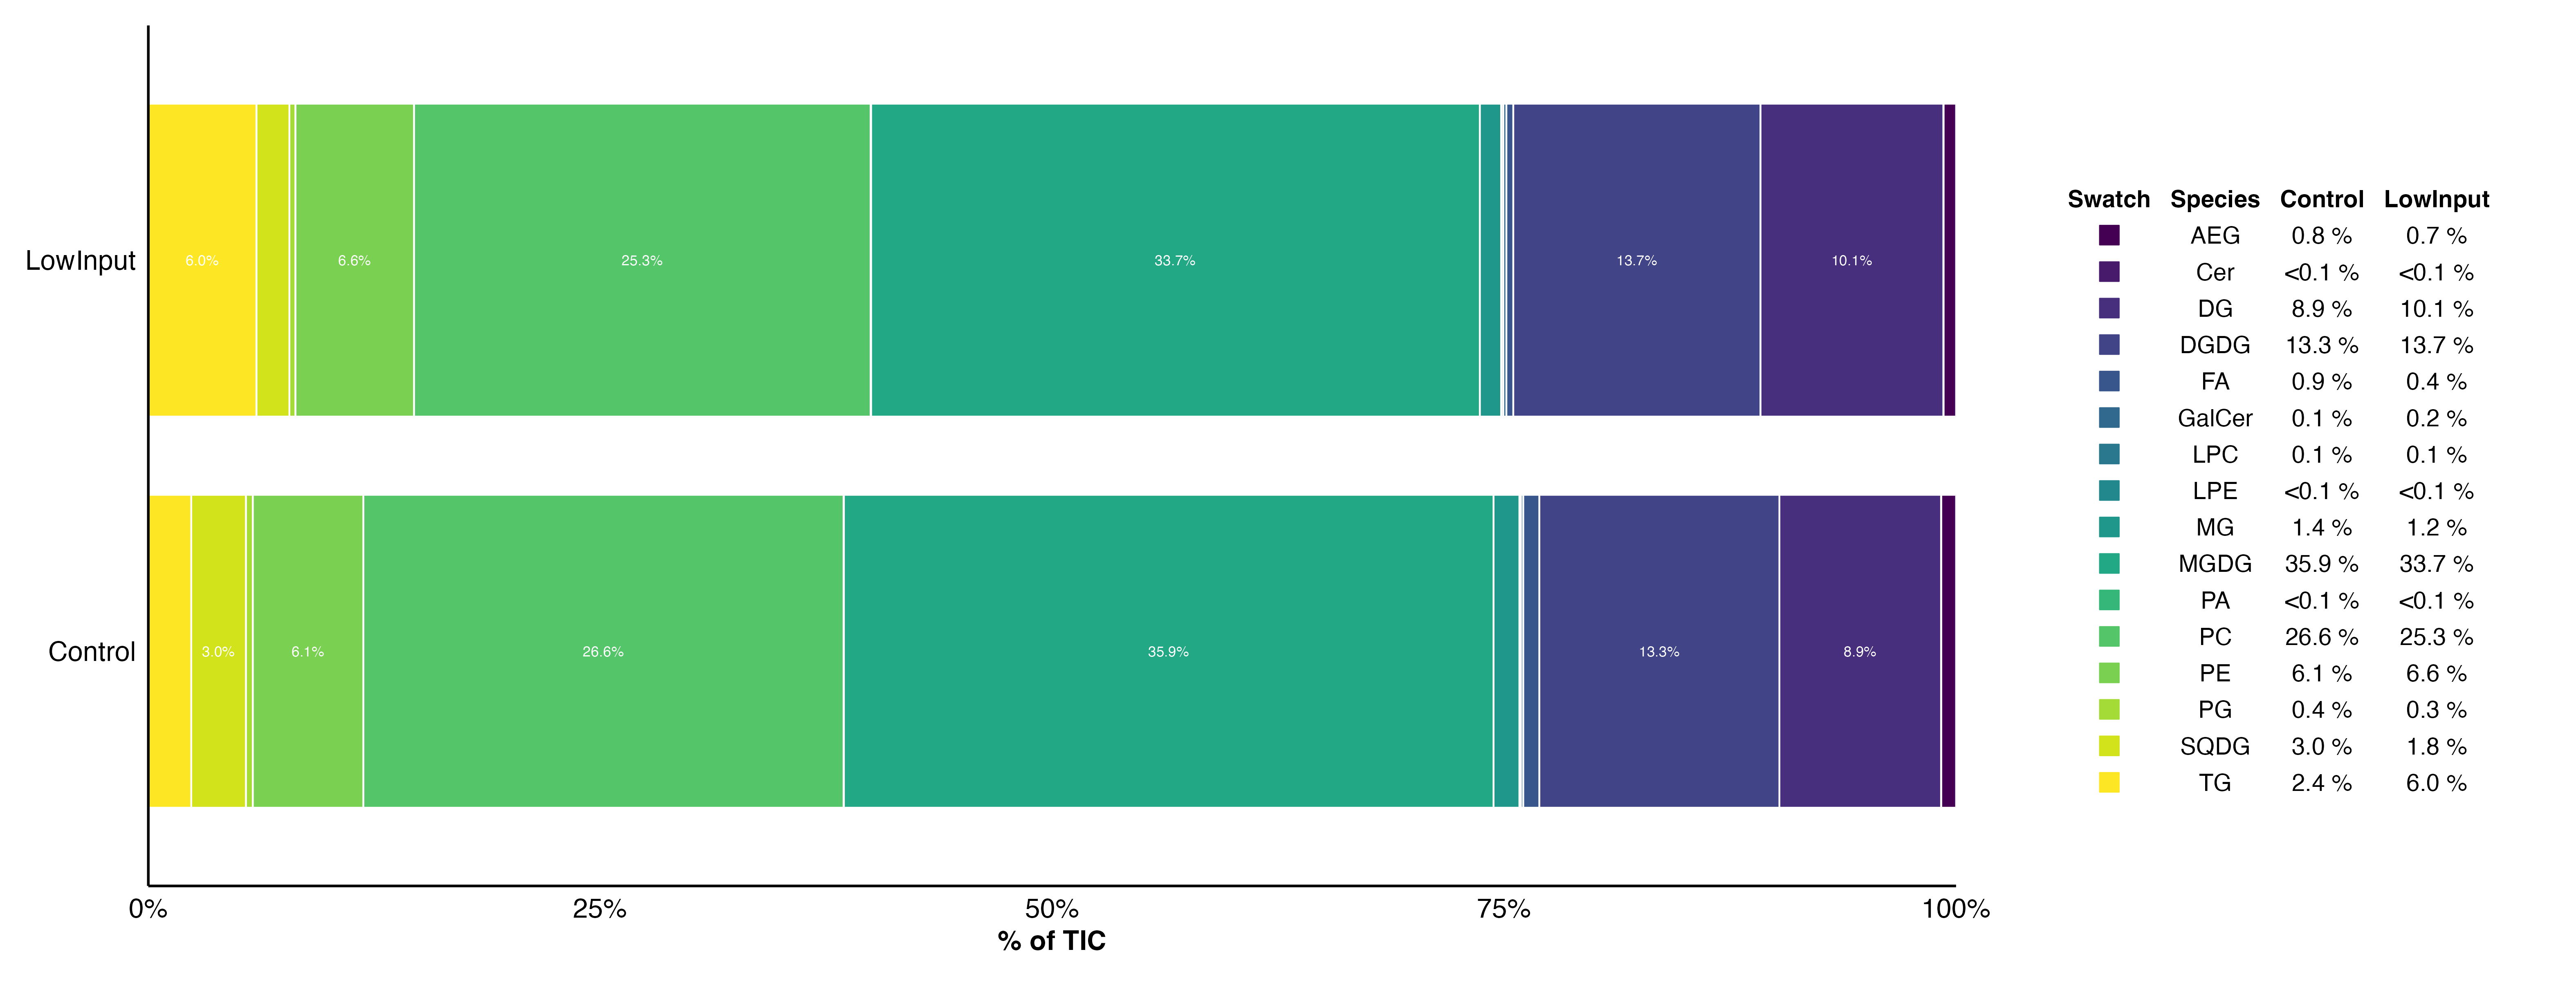
\includegraphics[width=\textwidth]{fig/main/Fig1a_lipid_species.png}
    \caption{Species‐level lipid composition (\% of TIC).}
    \label{fig:1A_lipid_species}
  \end{subfigure}

  \vspace{1em} % small vertical gap between panels

  %----------------------------------------------------
  %  (B) Bottom panel: class‐level lipid composition
  %----------------------------------------------------
  \begin{subfigure}[t]{\textwidth}
    \centering
    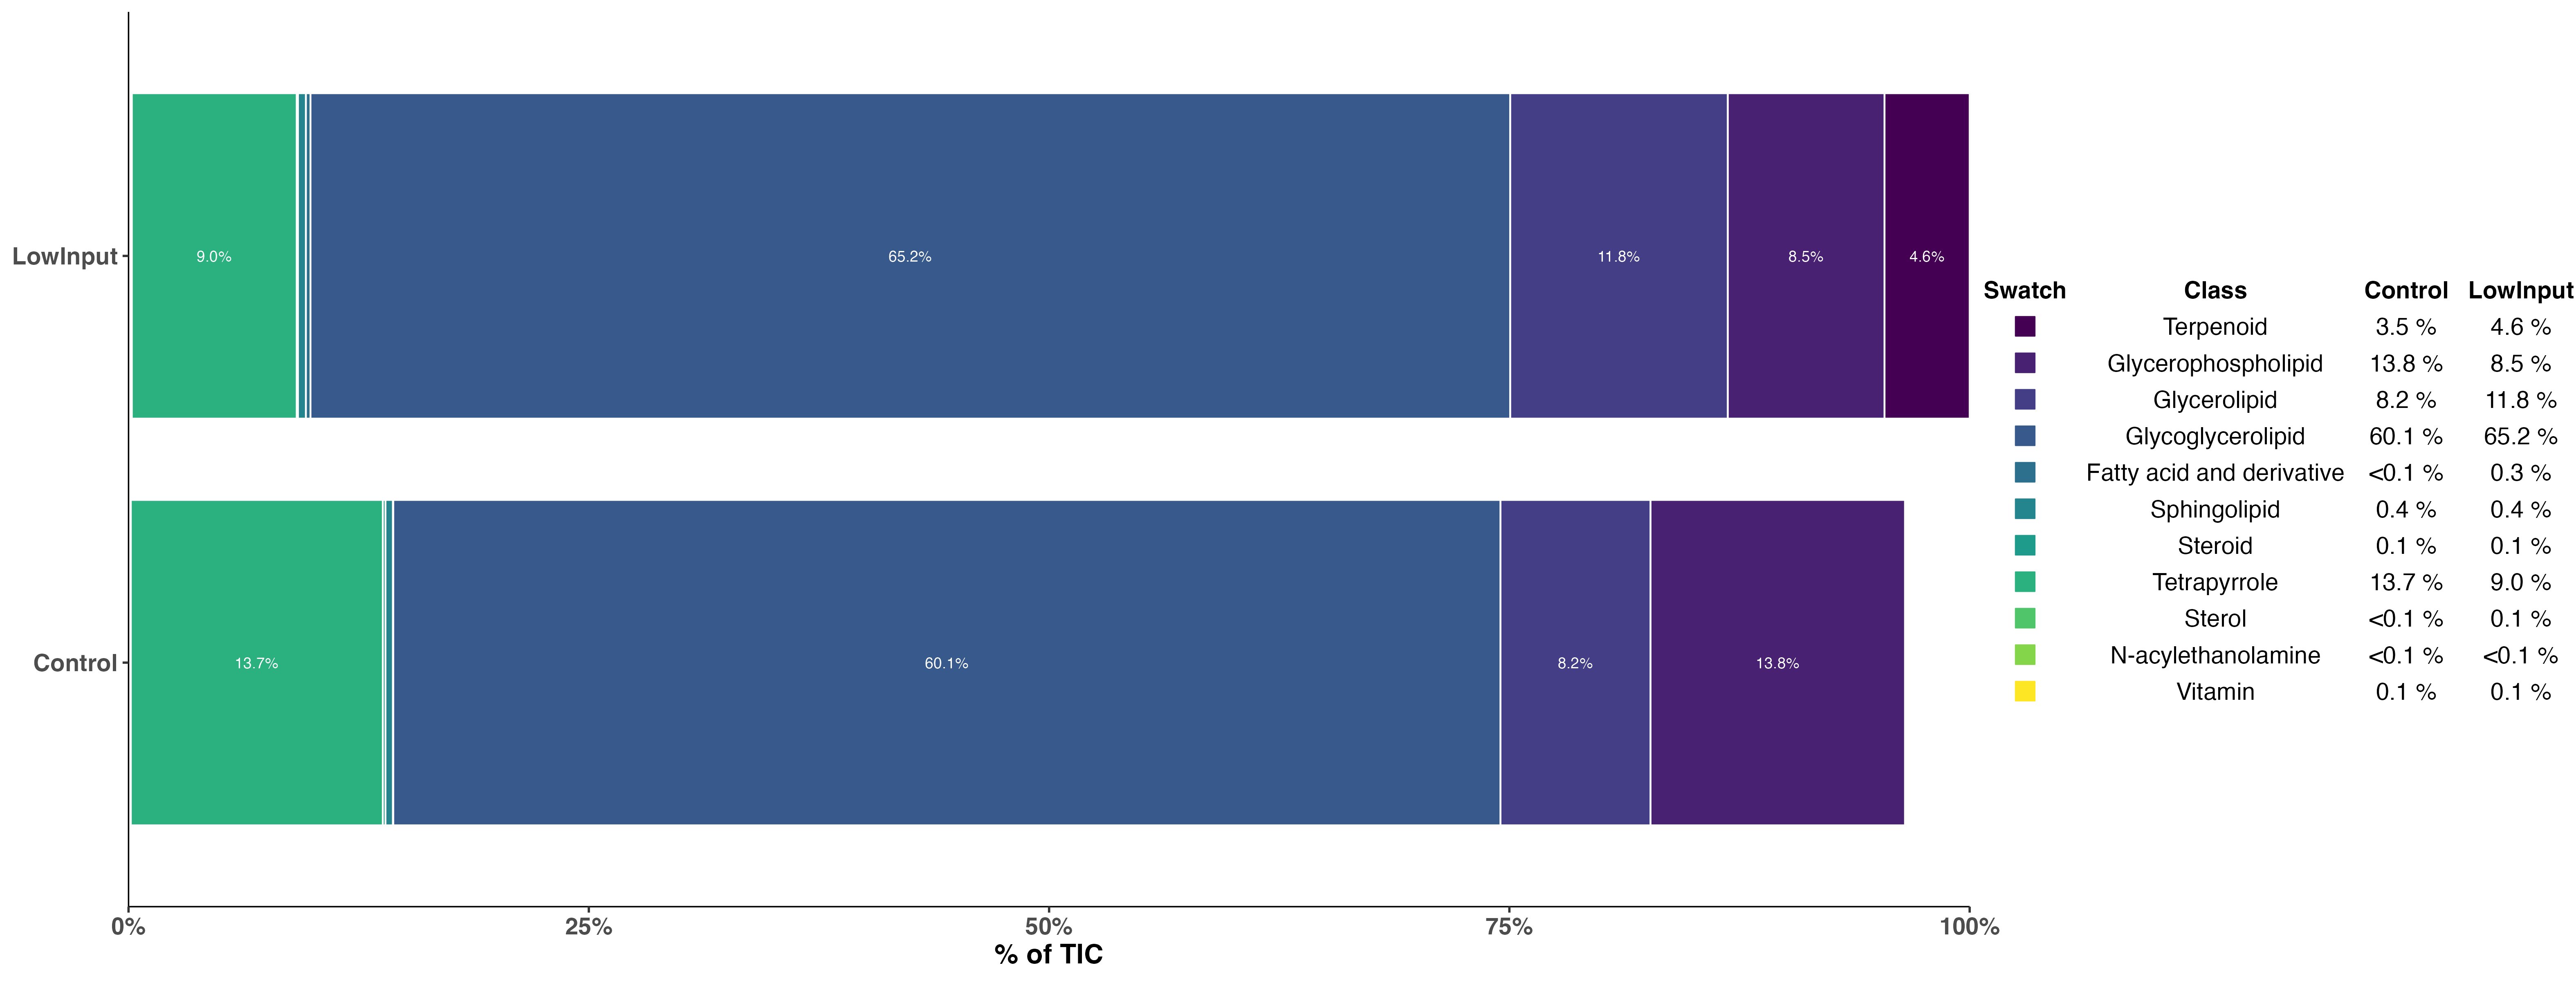
\includegraphics[width=\textwidth]{fig/main/Fig1b_lipid_class.png}
    \caption{Class‐level lipid composition (\% of TIC).}
    \label{fig:1B_lipid_class}
  \end{subfigure}

  \vspace{0.5em}

  \caption{%
    (A) Percent‐of‐TIC breakdown for individual lipid \emph{species}, averaged across all C (n = 384) and LI (n = 362) samples. Only species whose mean contribution ≥ 3 \% are labeled in‐bar.  
    (B) Percent‐of‐TIC breakdown for broader lipid \emph{classes} averaged across the same sets of samples.  
    In both panels, “Control” is shown in purple and “Low Input” in yellow.}
  \label{fig:lipid_main}
\end{figure}



\subsection*{Effect of low P condition on lipid composition: The limitation of P triggers the remodeling of the lipidome away from phospholipids}

\subsubsection*{Galactolipid Enrichment Characterizes the P Stress Response}
Under phosphorus deprivation, SAP lines exhibit a pronounced remodeling of membrane lipids characterized by a large shift from phospholipids to non-P galactolipids. This is evident from the markedly positive $\Delta$Z‐score contrasts for \texttt{DGDG/PC} and \texttt{MGDG/PE} (both $p<0.001$) as well as for \texttt{MGDG-PC} and \texttt{MGDG-PE} ($p<0.001$). These ratios increase substantially under low-P conditions, indicating that the diacylglycerol group preferentially routed to the synthesis of digalactosyldiacylglycerol and monogalactosyldiacylglycerol rather than toward phosphatidylcholine or phosphatidylethanolamine. This reallocation likely preserves bilayer stability and photosynthetic membrane function without sustaining the high P cost of maintaining large phospholipid pools (Fig. \ref{fig:2a_ratio_lowP}, first 4 panels).

Furthermore, the \texttt{non-P\_P\_total} metric: $((\mathrm{MGDG} + \mathrm{DGDG}) - (\mathrm{PC} + \mathrm{PE}))$ yields a large positive $\Delta$Z ($p<0.001$), confirming a global transition from P-containing lipids to P-free galactolipids. This reflects a broad replacement of phospholipids with galactolipids under P limitation (Fig. \ref{fig:2a_ratio_lowP}, last panel).

\subsubsection*{Selective Retention of Phosphatidylglycerol (PG)}
Despite the global shift to galactolipids, certain subclasses of phospholipids show selective conservation consistent with metabolic prioritization. The retention metric of PG: $(PG – (PC + PE)/2)$, shows a modest but significant change $\Delta Z$ ($p<0.05$), indicating that even as the overall phospholipid pools decline, PG is relatively conserved compared to PC and PE. The preservation of PG aligns with its essential role in thylakoid and photosynthetic membranes, implying that SAP lines maintain a minimal complement of PG under P stress (Fig. \ref{fig:2a_ratio_lowP}). 

\subsubsection*{Lysophospholipid Dynamics and Possible P Salvage}
Lysophospholipid change reveal insights into P recycling at low P. The $\Delta$Z for \texttt{LPC-PC} is not significant (Supp Fig. A), indicating that the balance between LPC and its parent PC remains broadly stable. In contrast, the $\Delta$Z for \texttt{LPE-PE} shows a modest but significant positive change ($p<0.01$, Supp. Fig. B), which implies an increase in the deacylation of PE to LPE under the limitation of P. The composite \texttt{Lyso\_activity} metric,defined as $((\mathrm{LPC} + \mathrm{LPE}) - (\mathrm{PC} + \mathrm{PE}))$, also shifts toward zero (i.e. less negative) under low P (Fig.~\ref{fig:2a_ratio_lowP}), indicating the net accumulation of lysophospholipids relative to total phospholipids. The accumulation of LPE signals increased deacylation. P salvage requires further cleavage of the phospho-glycerol bond or dephosphorylation of the headgroup, for example through phospholipase C or D activities (yielding phospho-headgroups or phosphatidic acid), followed by phosphatases that release Pi. The observed rise in \texttt{LPC-PC} suggests that PE is being targeted for deacylation, making it available for downstream headgroup cleavage and eventual phosphate release, while PC is more strongly protected from such hydrolysis. 

In support of this, TIC-based proportions show a drop in the fraction of LPC and a rise in LPE under low P (Supp. Fig. X). Together, these findings indicate that SAP lines prioritize the preservation of PC integrity, which is critical to membrane stability and function, while channeling PE into a multistep salvage pathway to possibly free phosphate when required (Fig.~\ref{fig:2a_ratio_lowP}).

\subsection*{Limited Role of Sulfolipids in P Compensation}
Sulfolipid contrasts reveal that SQDG does not play a primary compensatory role P in SAP leaves under P deprivation. We define a \texttt{SQDG\_spared} metric as $(\mathrm{SQDG} - (\mathrm{DGDG} + \mathrm{MGDG} + \mathrm{PG}))$ ,which assesses whether SQDG levels are maintained (positive $\Delta$Z) or drawn down (negative $\Delta$Z) relative to the main galactolipids and PG. In our data, the $\Delta$Z contrast for \texttt{SQDG\_Spared} is significantly negative ($p<0.001$, Supp Fig.~X), indicating that under low P, SQDG declines more (or is less preserved) compared to the average levels of DGDG, MGDG and PG. This contrasts with systems where SQDG substitutes for PG under P starvation. In our multistress environment, SAP lines are primarily based on galactolipid enrichment plus selective PG retention without upregulating SQDG. The negative shift in \texttt{SQDG\_Spared} suggests that maintaining the balance of membrane charge and photosynthetic function is achieved through increased synthesis of DGDG / MGDG and conservation of PG, making up-regulation of SQDG unnecessary.

%==========================================
%  Figure 2A – Lipid-class ratios under LI
%==========================================
\begin{figure}[htbp]
  \centering
  % Use a tabular with two columns for precise control
  \begin{tabular}{@{}p{0.33\textwidth}@{\hspace{1em}}p{0.63\textwidth}@{}}
    % Left: (a) in a minipage for top alignment
    \begin{minipage}[t]{\linewidth}
      \vspace{0pt} % ensures top alignment baseline
      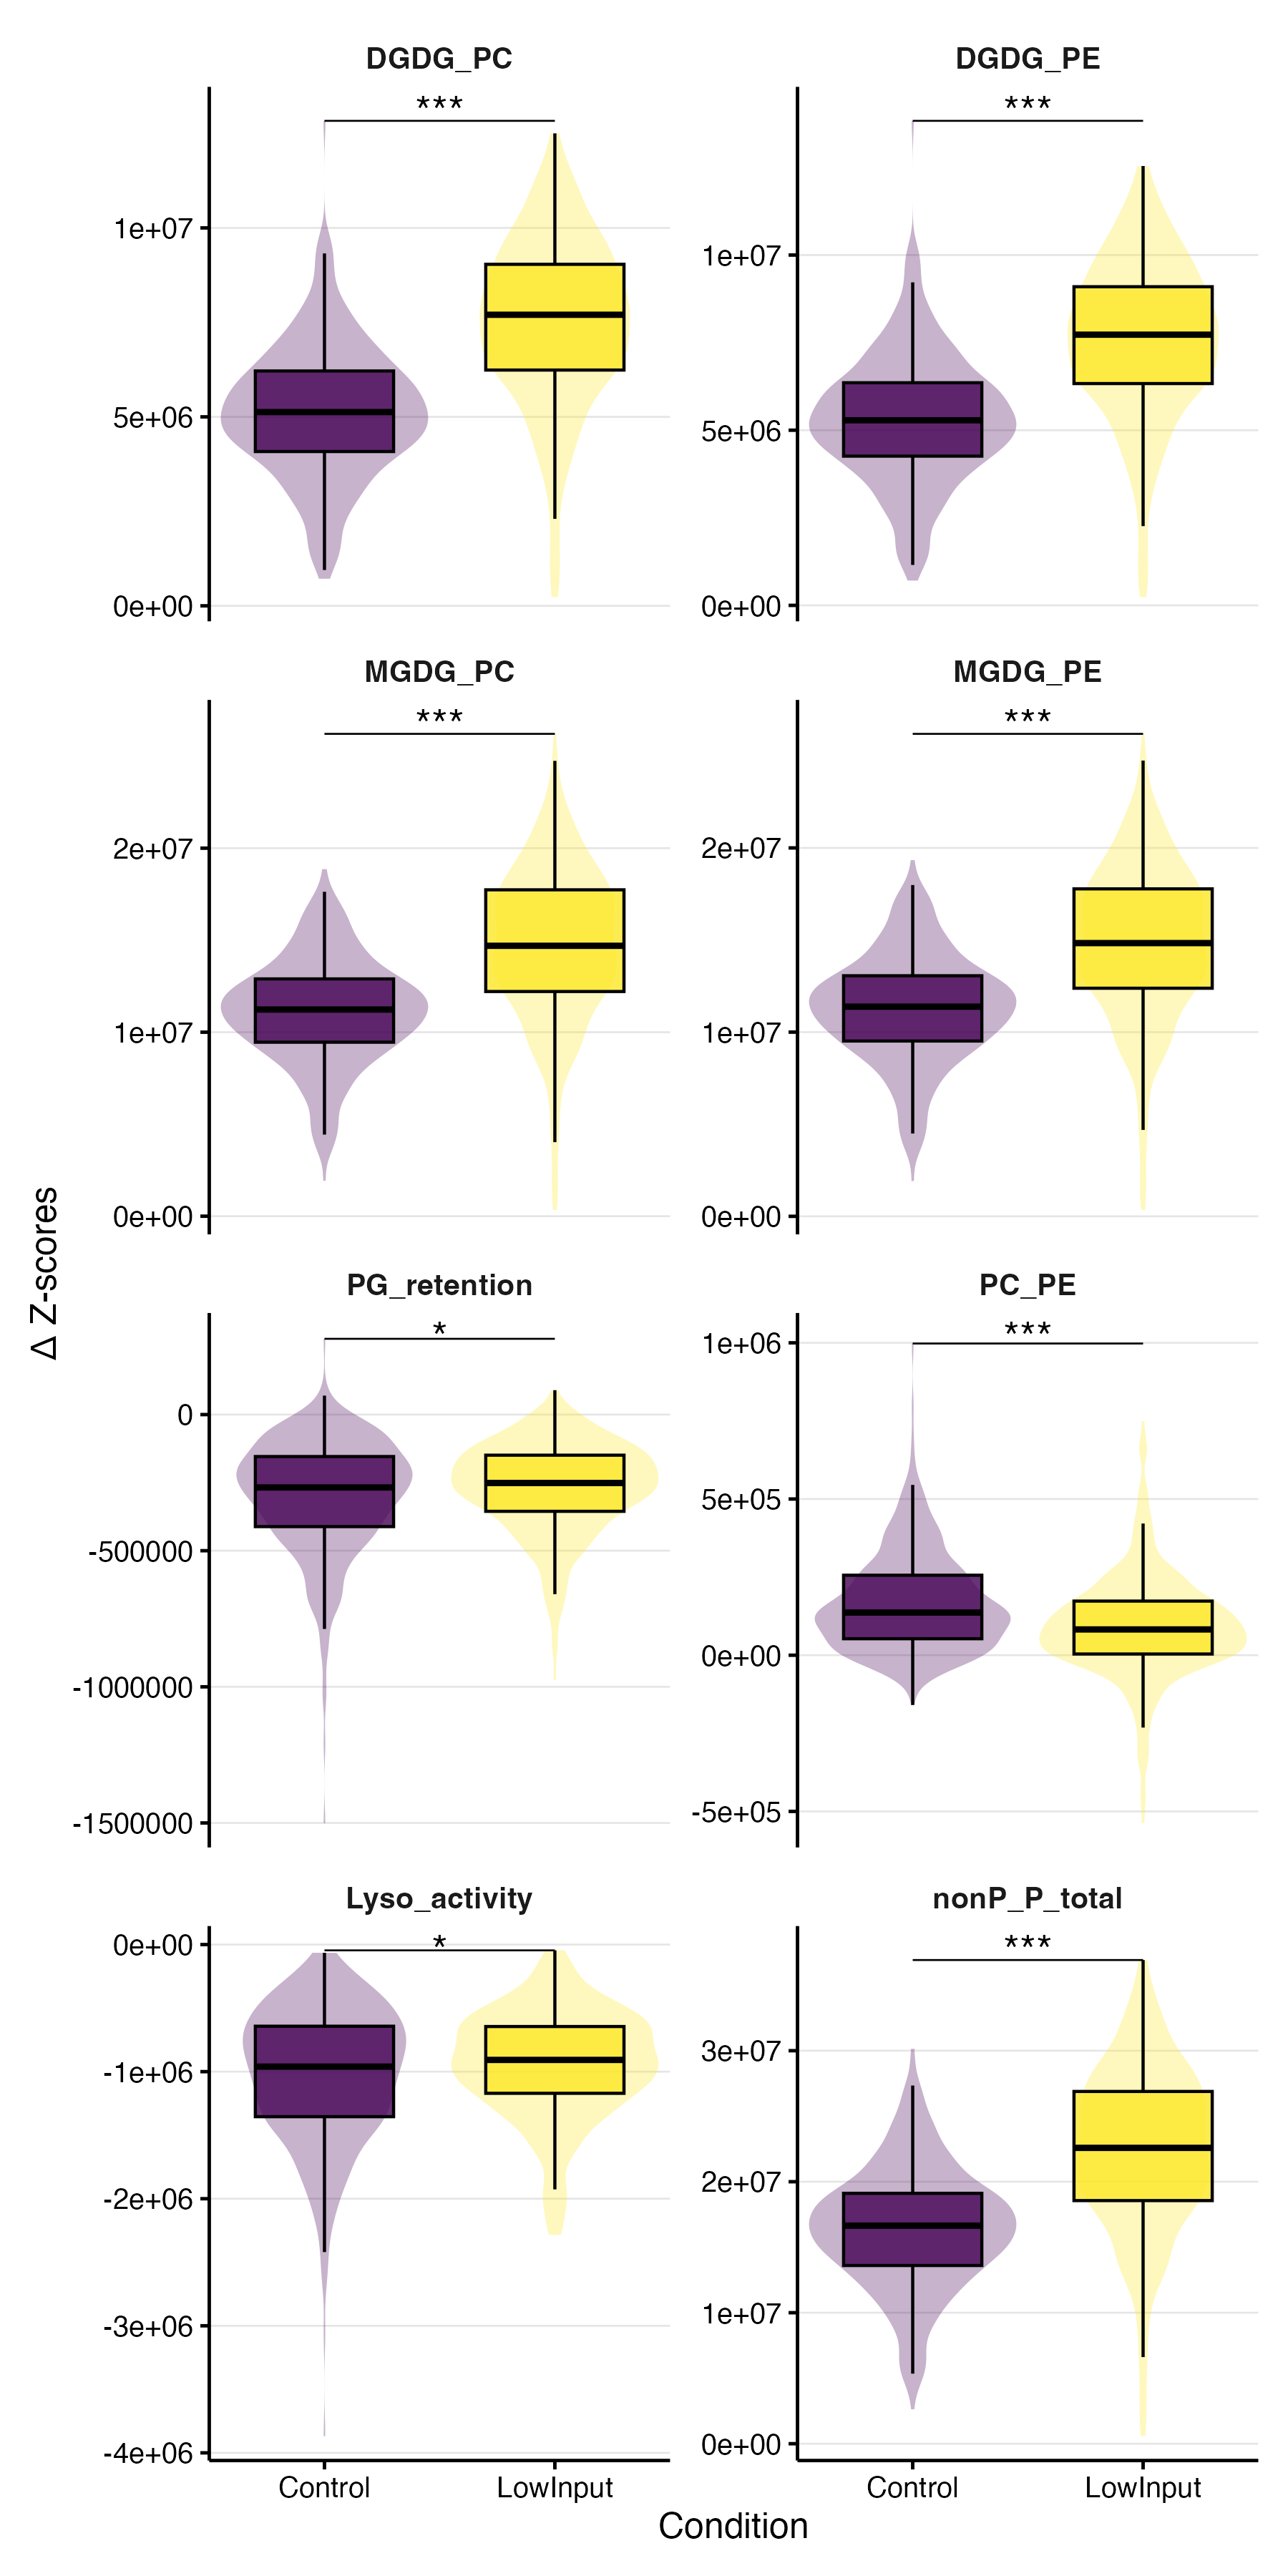
\includegraphics[width=\linewidth]{fig/main/Fig2a_lipid_ratio_linear_lowP.png}
      \subcaption{Lipid-class ratios under P deprivation (Low-P).}
      \label{fig:2a_ratio_lowP}
    \end{minipage}
    &
    % Right: a vertical box stacking (b) and (c)
    \begin{minipage}[t]{\linewidth}
      \vspace{0pt}
      % Top: (b)
      \begin{minipage}[t]{\linewidth}
        \vspace{0pt}
        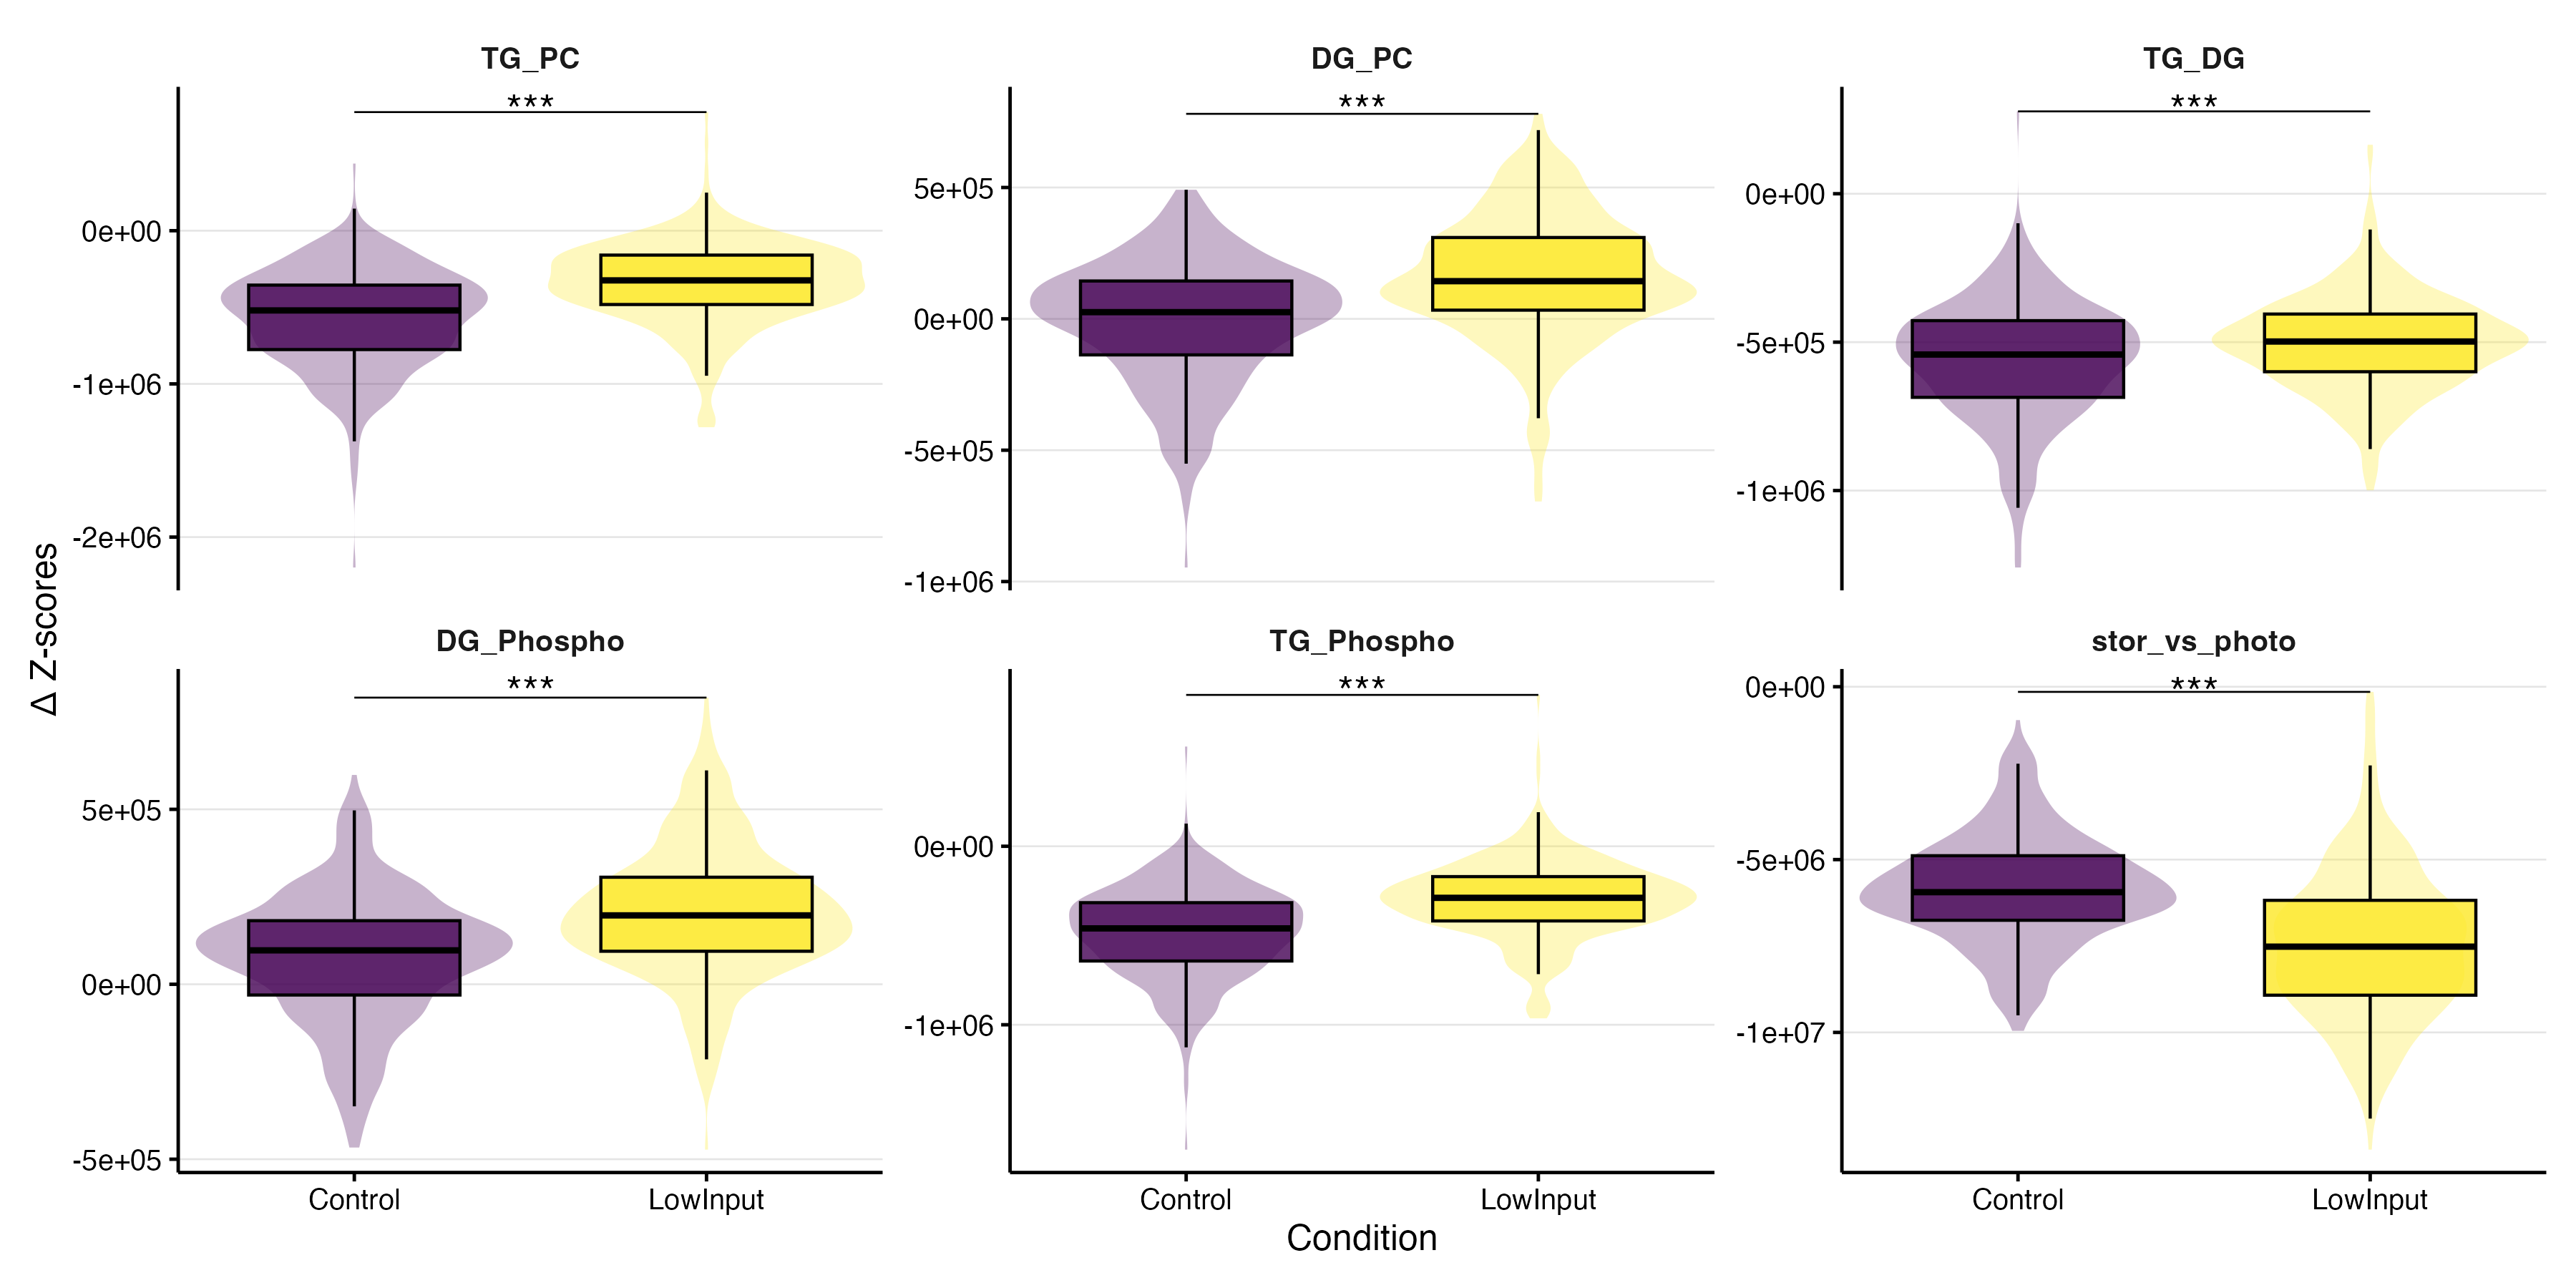
\includegraphics[width=\linewidth]{fig/main/Fig2b_lipid_ratio_linear_lowN.png}
        \subcaption{Lipid-class ratios under N deprivation (Low-N).}
        \label{fig:2b_ratio_lowN}
      \end{minipage}
      \\[1ex]
      % Bottom: (c)
      \begin{minipage}[t]{\linewidth}
        \vspace{0pt}
        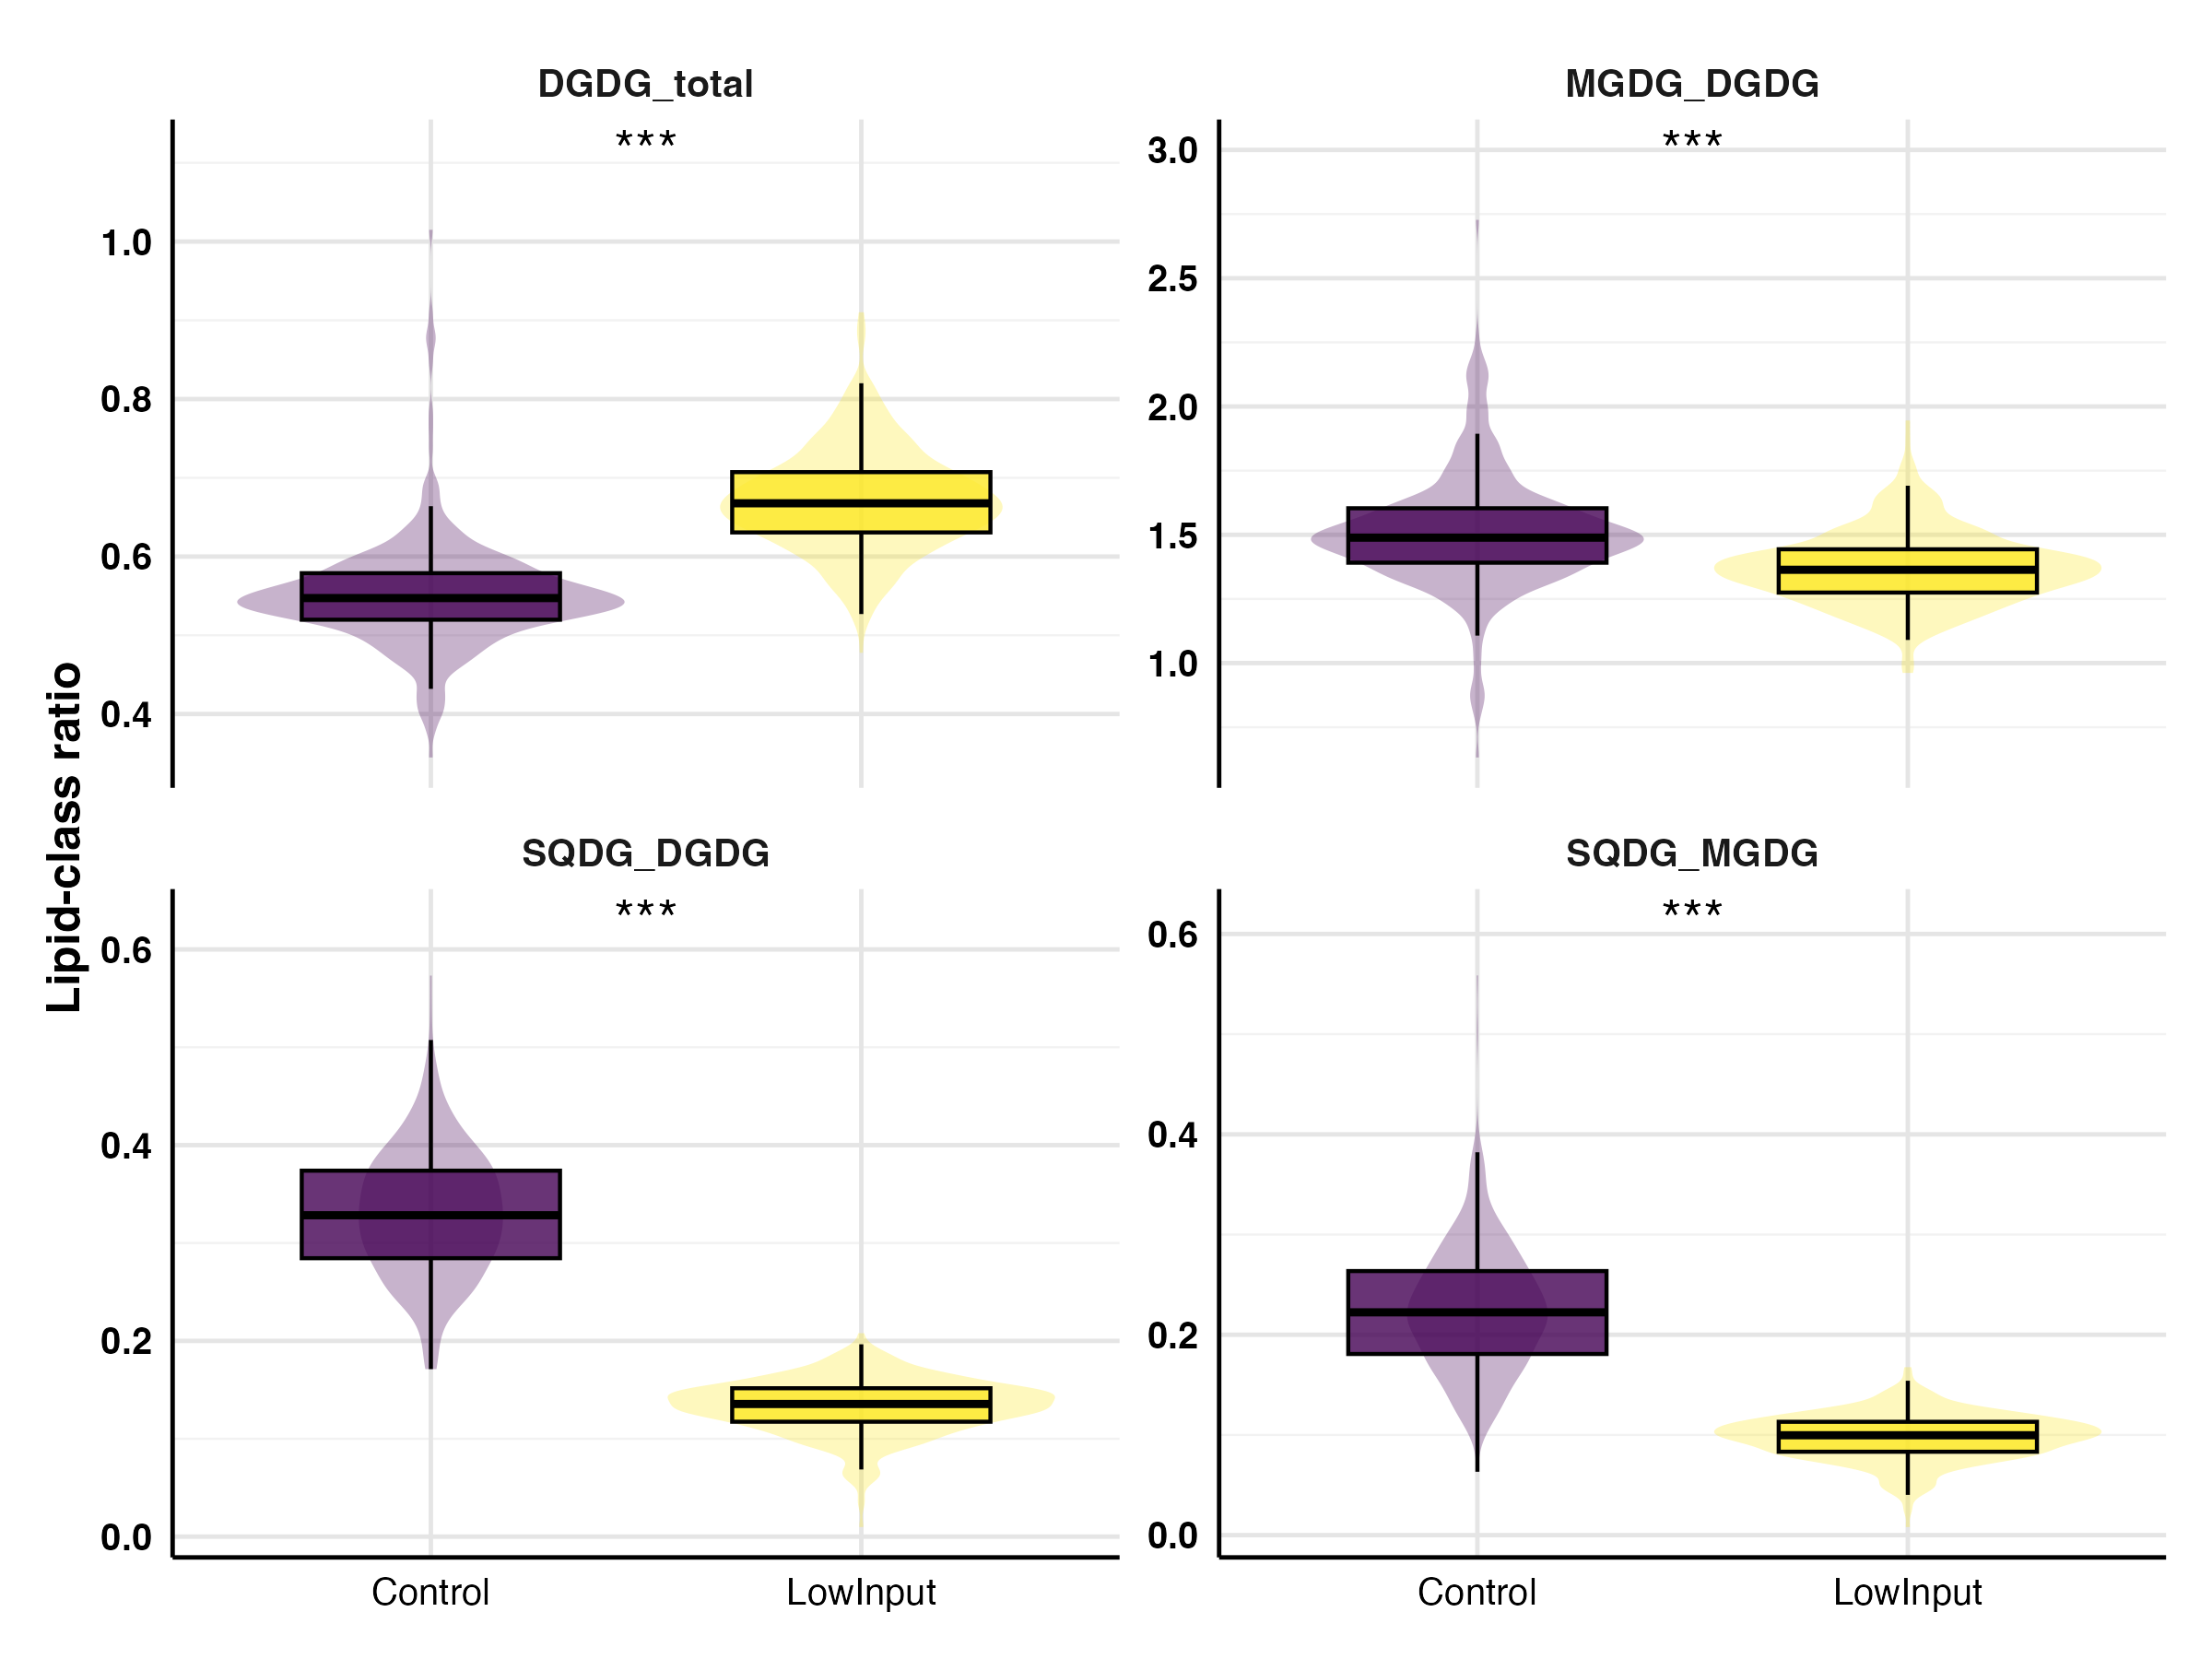
\includegraphics[width=\linewidth]{fig/main/Fig2c_lipid_ratio_linear_cold.png}
        \subcaption{Lipid-class ratios under cold stress.}
        \label{fig:2c_ratio_cold}
      \end{minipage}
    \end{minipage}
  \end{tabular}
  \caption{Overall lipid-class ratio comparisons under different conditions.}
  \label{fig:2_lipid_ratios}
\end{figure}



\subsection*{Effect of Low N condition on lipid composition: Nitrogen Limitation Triggers a Metabolic Shift from Membrane to Storage Lipids}

Under N deprivation, sorghum exhibits coordinated lipidomic reprogramming that redirects membrane lipid precursors toward neutral lipid accumulation. The $\Delta Z$ scores reveal that phospholipid degradation products accumulate and funnel into TG synthesis, a hallmark of the N stress response.

\subsubsection*{Membrane Phospholipid Breakdown Fuels Neutral Lipid Synthesis}

The \textit{DG/PC} and \textit{DG/Phospho} ratios increase significantly ($p < 0.001$), indicating that DG accumulates relative to both PC and the major phospholipid pool. This suggests either enhanced deacylation of phospholipids via phospholipase activity or a downregulation of PC biosynthesis. These freed DG molecules are not inert: both \textit{TG/DG} and \textit{TG/PC} ratios also shift upward ($p < 0.001$), showing that DG is actively esterified into TG. Thus, membrane phospholipids act as carbon and nitrogen donors releasing N from their headgroups and supplying DG backbones that are repurposed for energy storage.

\subsubsection*{Photosynthetic vs. Storage Lipid Trade-Off}

The composite \textit{stor\_vs\_photo} ratio contrasting TG + DG against photosynthetic lipids (MGDG + PC) rises sharply ($p < 0.001$), indicating a systemic reallocation from membrane expansion to carbon storage. This supports the notion that, under N stress, photosynthetic membrane development slows and photoassimilated carbon is redirected to neutral lipids. Such rebalancing is metabolically strategic: It prevents sugar overload when N-dependent biosynthetic pathways (e.g. amino acids, nucleotides) are suppressed, and stores excess carbon as TG for future remobilization.




\subsection*{Effect of cold condition on lipid composition: Cold Acclimation Remodels Galactolipid Composition in Sorghum Leaves}

Under cold stress, sorghum leaves exhibit a reconstruction of their galactolipid profile, as evidenced by significant shifts in all four $\Delta$Z ratios for DGDG\_total, MGDG\_DGDG, SQDG\_DGDG, and SQDG\_MGDG (all p < 0.001). The three major nonphosphorous glycerolipids, DGDG, MGDG, and SQDG, most likely confer the adaptation to low temperature.

\paragraph{Galactolipid boost (DGDG_total).}
Cold stress markedly increases the overall contribution of DGDG to the non‑P lipid pool. The $\mathrm{DGDG}_{\mathrm{total}}$ contrast shifts strongly positive ($\Delta Z \gg 0$ ; $p < 0.001$). A larger DGDG fraction is a classic response that helps preserve bilayer order at low temperature while avoiding the need for phosphorus.

\paragraph{Curvature tuning via MGDG enrichment (MGDG_DGDG).}
The MGDG_DGDG ratio also increases ($\Delta Z \gg 0$ ; $p < 0.001$), indicating that monogalactosyldiacylglycerol (MGDG) increases even faster than DGDG. Because MGDG is a non‑bilayer–forming lipid that promotes membrane flexibility, its enrichment relative to DGDG likely fine‑tunes thylakoid curvature and counteracts cold‑induced rigidity.

\paragraph{Sulfolipid down‑shift (SQDG_DGDG and SQDG_MGDG).}
Both sulfolipid contrasts move decisively downward ($\Delta Z \gg 0$ ; $p < 0.001$), showing that sulfoquinovosyldiacylglycerol (SQDG) becomes relatively scarcer than either galactolipid under cold. The absolute TIC data corroborate the trend (SQDG falls to 11. 7\% 5. 3\%). Rather than increasing the anionic lipid content, sorghum cold acclimation favors neutral galactolipids and simultaneously trims SQDG, perhaps to avoid an excessive negative surface charge or to redirect sulfur to other stress pathways.

Taken together, cold acclimation in sorghum does not mimic the SQDG up‑regulation reported for some species. Instead, it relies on a concerted galactolipid re‑balancing—boosting DGDG and, even more, MGDG—to maintain membrane fluidity, while deliberately curbing SQDG. The highly consistent, non‑overlapping violin distributions confirm that this remodeling is systematic across replicates and constitutes a key feature of the sorghum cold‑stress response.




\subsection*{Multivariate structure of lipid profiles}

\subsection*{Genome-wide association study (GWAS) of lipids}

\subsection*{Pathway identification}



%--------------------------------------------------------------------
\bibliographystyle{plainnat}
\bibliography{lipid_refs}



\section*{Discussion}
Something something lipids are good. 


\section*{Conclusion}

because we can For more information, see \nameref{S1_Appendix}.

\section*{Supporting information}

% Include only the SI item label in the paragraph heading. Use the \nameref{label} command to cite SI items in the text.
\paragraph*{S1 Fig.}
\label{S1_Fig}
{\bf Bold the title sentence.} Add descriptive text after the title of the item (optional).

\paragraph*{S2 Fig.}
\label{S2_Fig}
{\bf Lorem ipsum.} Maecenas convallis mauris sit amet sem ultrices gravida. Etiam eget sapien nibh. Sed ac ipsum eget enim egestas ullamcorper nec euismod ligula. Curabitur fringilla pulvinar lectus consectetur pellentesque.

\paragraph*{S1 File.}
\label{S1_File}
{\bf Lorem ipsum.}  Maecenas convallis mauris sit amet sem ultrices gravida. Etiam eget sapien nibh. Sed ac ipsum eget enim egestas ullamcorper nec euismod ligula. Curabitur fringilla pulvinar lectus consectetur pellentesque.

\paragraph*{S1 Video.}
\label{S1_Video}
{\bf Lorem ipsum.}  Maecenas convallis mauris sit amet sem ultrices gravida. Etiam eget sapien nibh. Sed ac ipsum eget enim egestas ullamcorper nec euismod ligula. Curabitur fringilla pulvinar lectus consectetur pellentesque.

\paragraph*{S1 Appendix.}
\label{S1_Appendix}
{\bf Lorem ipsum.} Maecenas convallis mauris sit amet sem ultrices gravida. Etiam eget sapien nibh. Sed ac ipsum eget enim egestas ullamcorper nec euismod ligula. Curabitur fringilla pulvinar lectus consectetur pellentesque.

\paragraph*{S1 Table.}
\label{S1_Table}
{\bf Lorem ipsum.} Maecenas convallis mauris sit amet sem ultrices gravida. Etiam eget sapien nibh. Sed ac ipsum eget enim egestas ullamcorper nec euismod ligula. Curabitur fringilla pulvinar lectus consectetur pellentesque.

\section*{Acknowledgments}
Me, myself and I

\nolinenumbers

% Either type in your references using
% \begin{thebibliography}{}
% \bibitem{}
% Text
% \end{thebibliography}
%
% or
%
% Compile your BiBTeX database using our plos2015.bst
% style file and paste the contents of your .bbl file
% here. See http://journals.plos.org/plosone/s/latex for 
% step-by-step instructions.
% 
\begin{thebibliography}{10}

\bibitem{bib1}
Conant GC, Wolfe KH.
\newblock {{T}urning a hobby into a job: how duplicated genes find new
  functions}.
\newblock Nat Rev Genet. 2008 Dec;9(12):938--950.

\bibitem{bib2}
Ohno S.
\newblock Evolution by gene duplication.
\newblock London: George Alien \& Unwin Ltd. Berlin, Heidelberg and New York:
  Springer-Verlag.; 1970.

\bibitem{bib3}
Magwire MM, Bayer F, Webster CL, Cao C, Jiggins FM.
\newblock {{S}uccessive increases in the resistance of {D}rosophila to viral
  infection through a transposon insertion followed by a {D}uplication}.
\newblock PLoS Genet. 2011 Oct;7(10):e1002337.

\end{thebibliography}

%==========================================
%   Start the Supplementary Material section
%==========================================
\FloatBarrier
\section*{Supplementary Material}
\beginsupplement


%========================================================
%  Supplementary Figure S1 – TIC traces
%========================================================
\begin{figure}[htp]
  \centering

  % ---------- panel A: Control TIC ----------
  \begin{subfigure}[t]{\textwidth}
    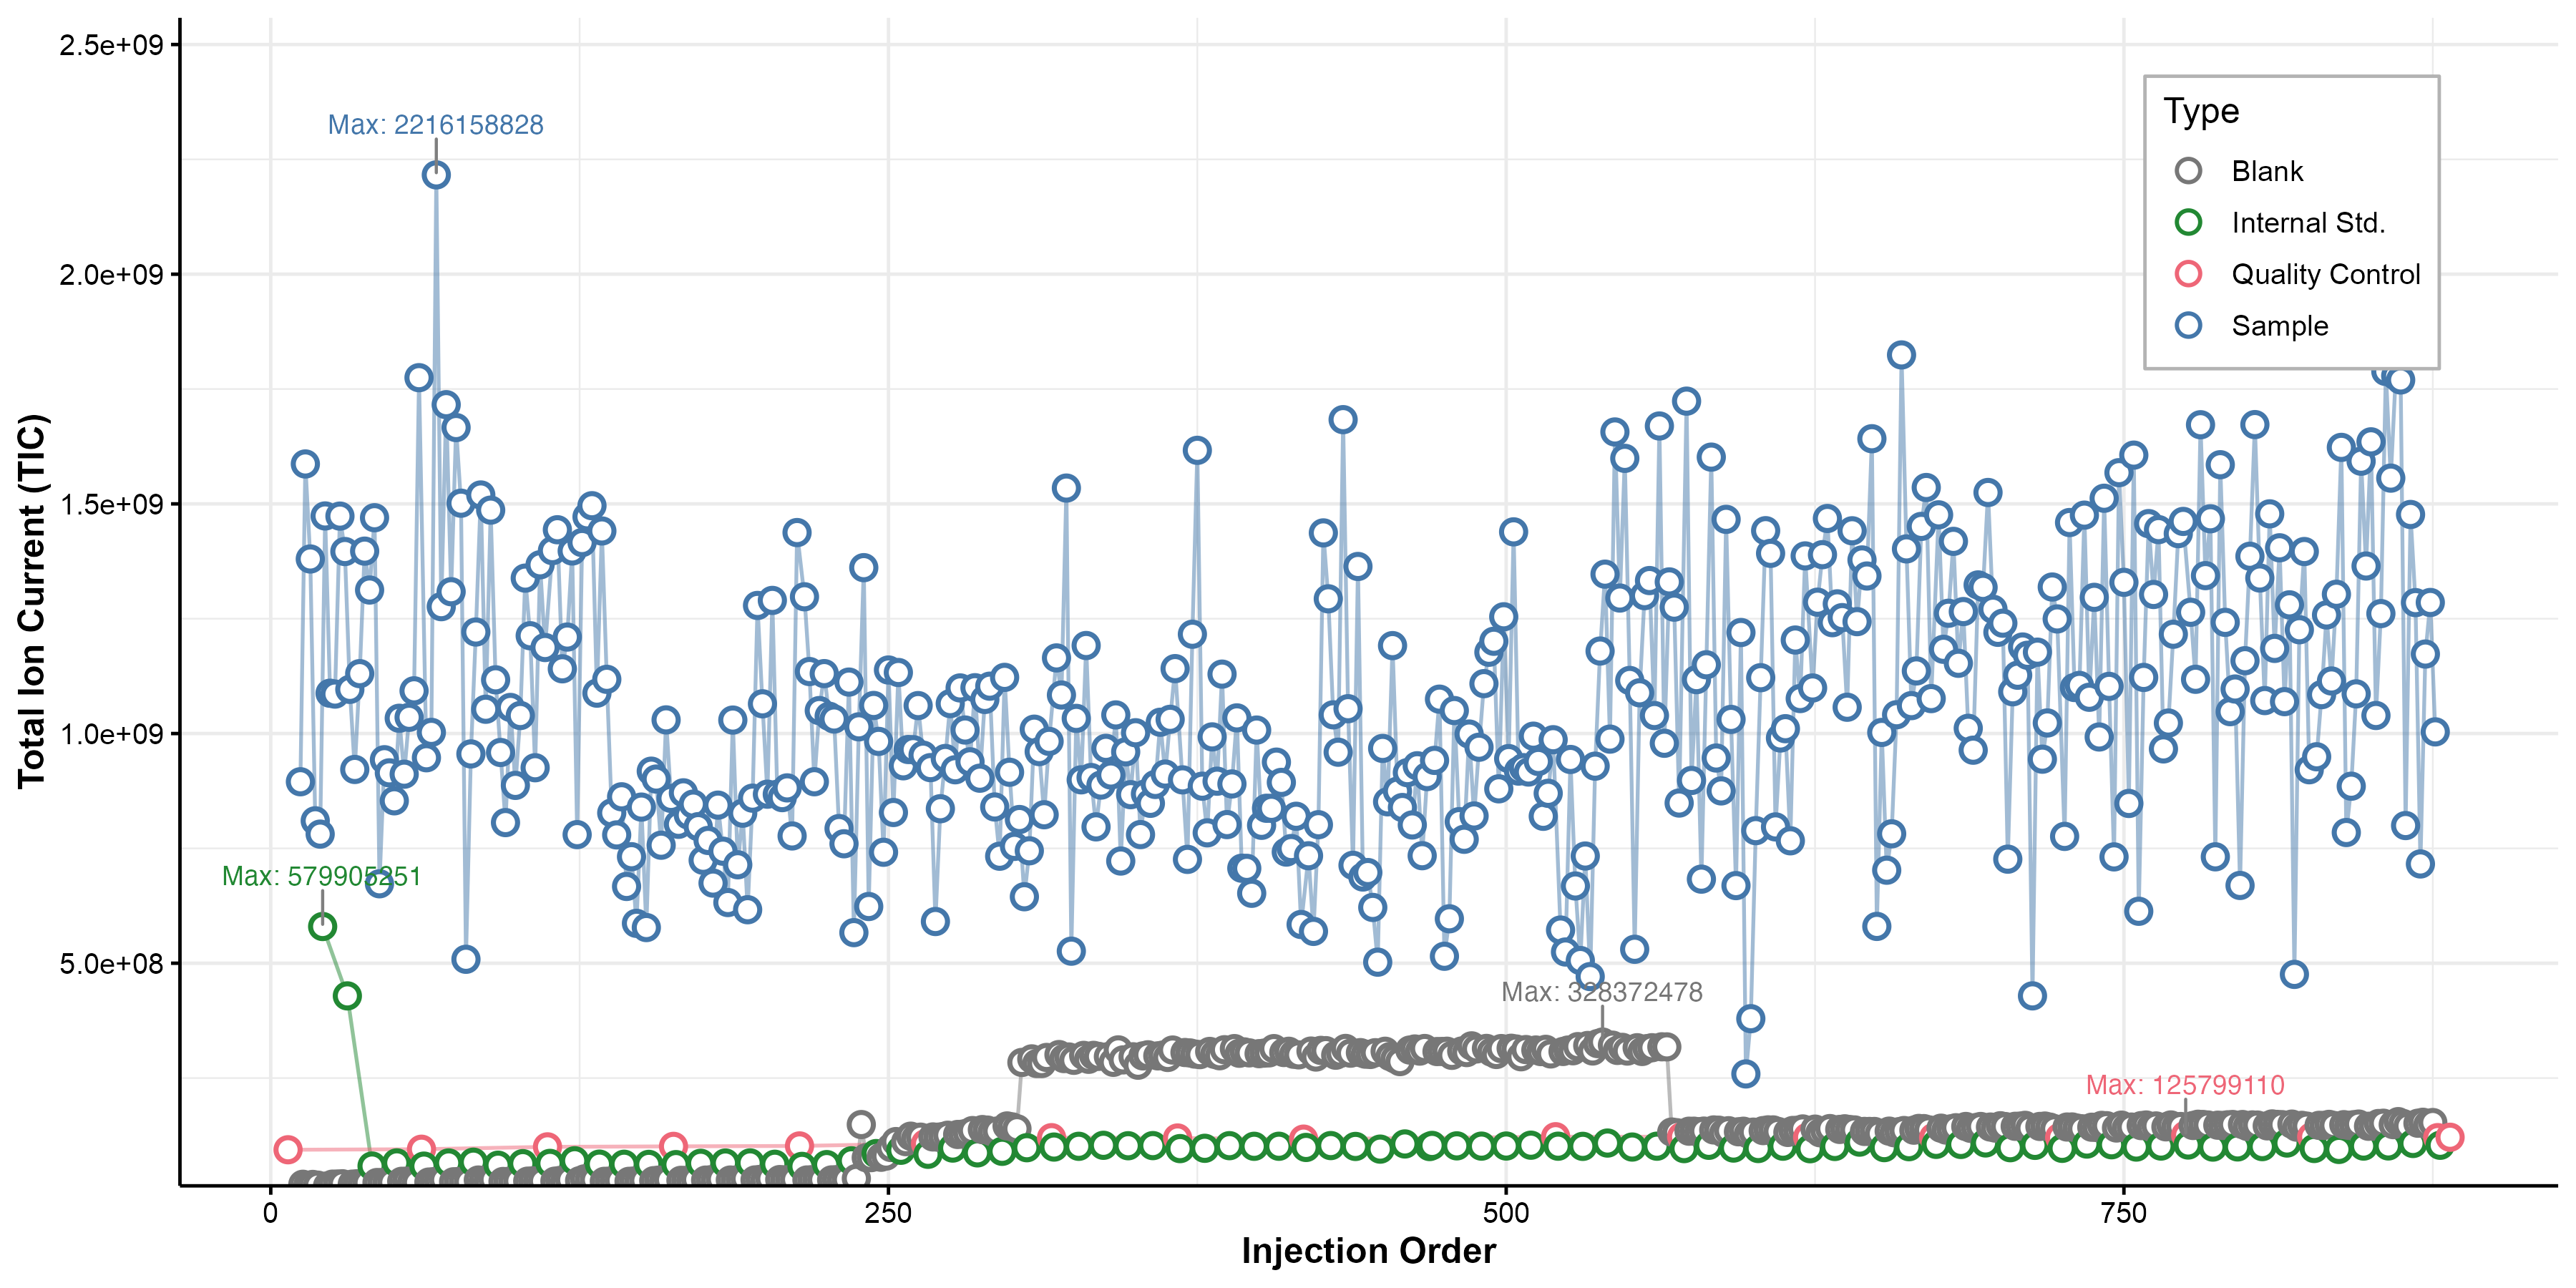
\includegraphics[width=\linewidth]{fig/supp/SuppFig_1A_TIC_Control}
    \caption{Total ion current vs.\ injection order for Control samples.}
    \label{fig:S1A}
  \end{subfigure}

  \vspace{1em}

  % ---------- panel B: Low-Input TIC ----------
  \begin{subfigure}[t]{\textwidth}
    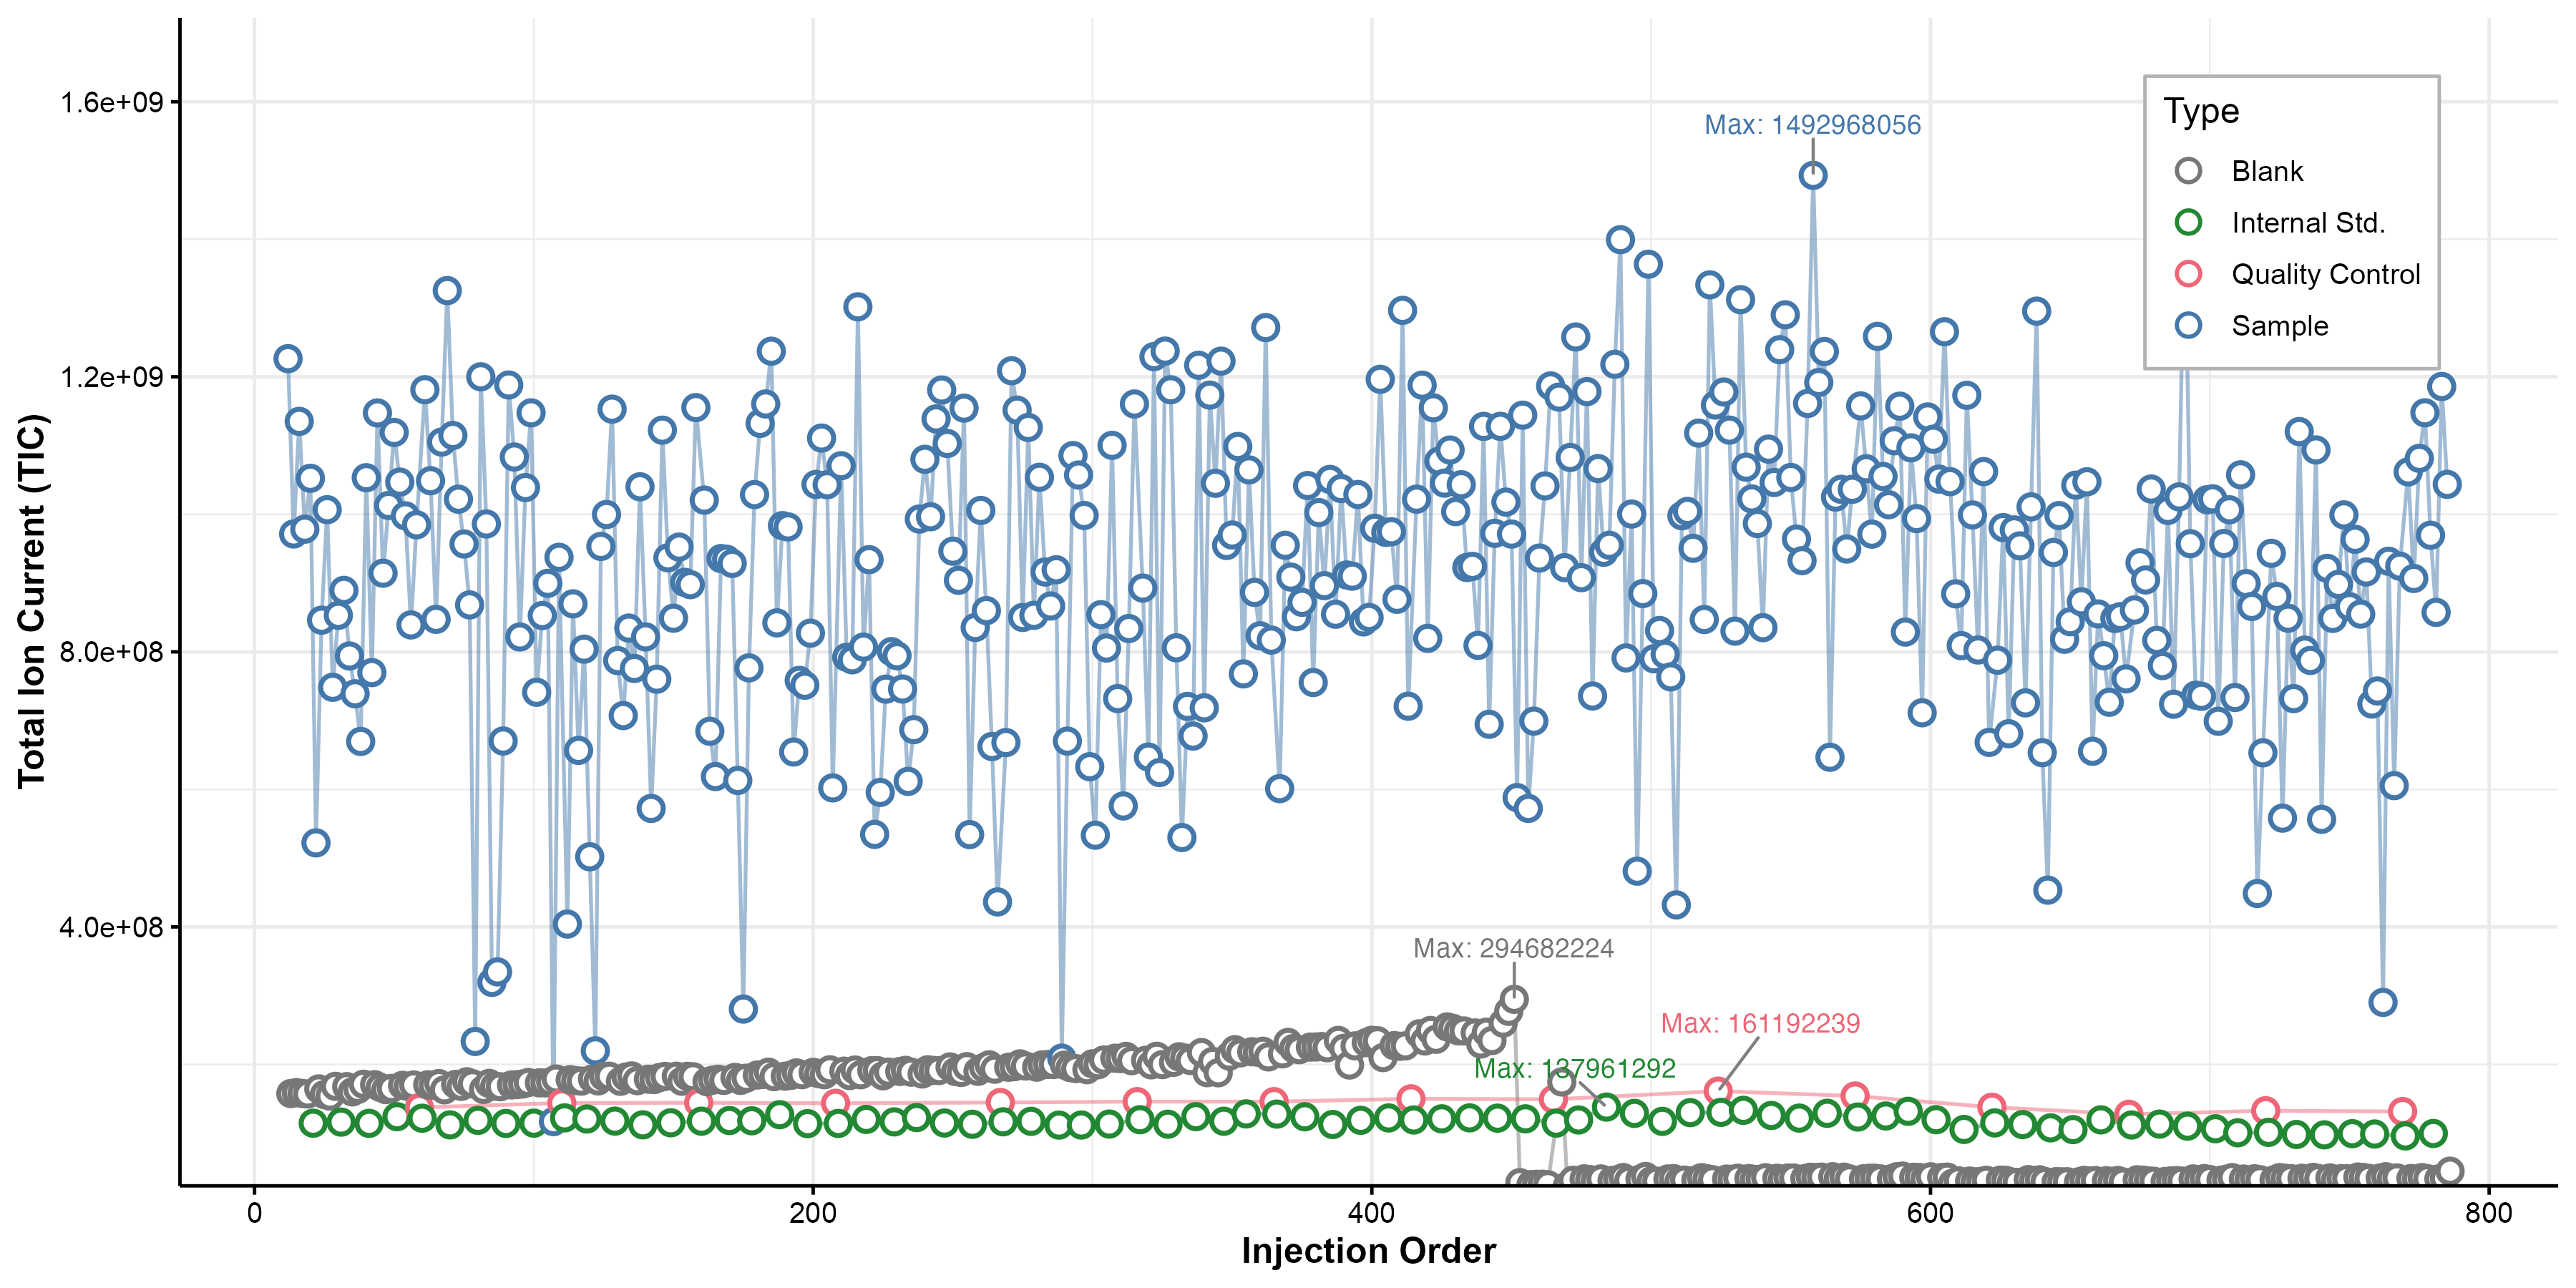
\includegraphics[width=\linewidth]{fig/supp/SuppFig_1B_TIC_LowInput.png}
    \caption{Total ion current vs.\ injection order for Low-Input samples.}
    \label{fig:S1B}
  \end{subfigure}

  \caption{TIC traces for all injections.  (A) Control, (B) Low-Input.}
  \label{fig:S1}
\end{figure}



%========================================================
%  Supplementary Figure S2 - SERFF RSD & PCA results
%========================================================
\begin{figure}[htp]
  \centering

  % ---------- row 1 ----------
  \begin{subfigure}[t]{0.48\textwidth}
    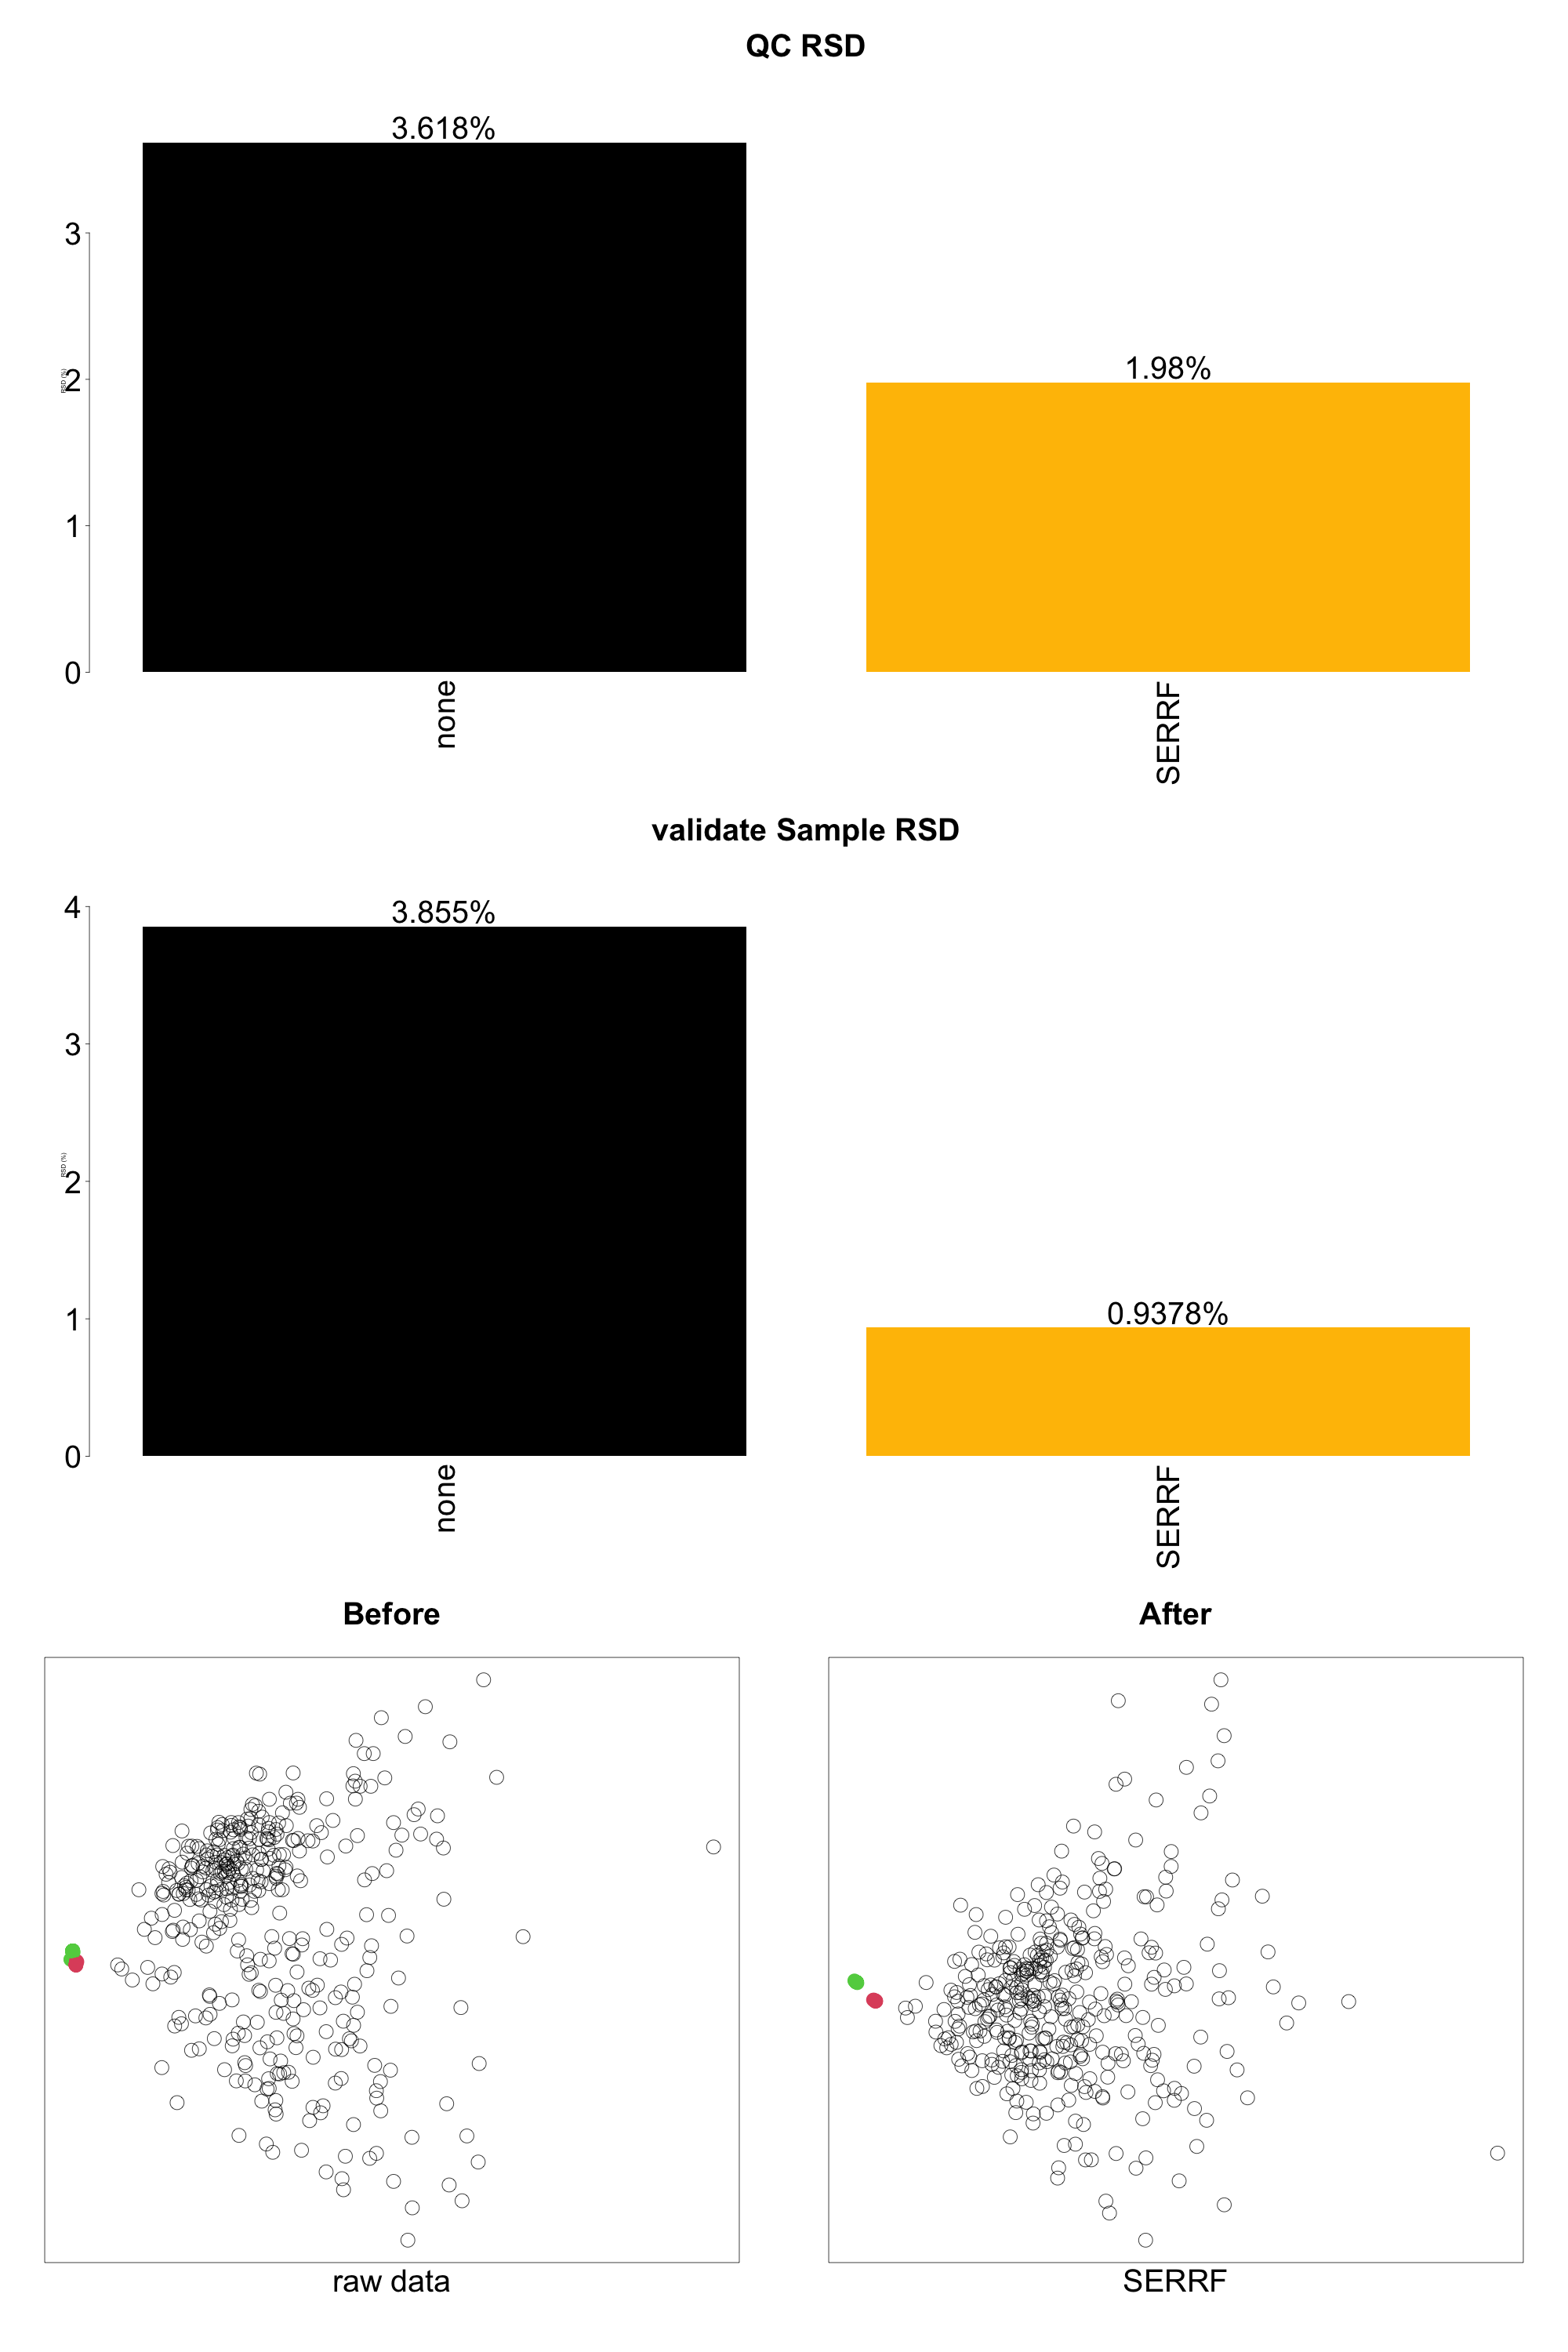
\includegraphics[width=\linewidth]{fig/supp/SuppFig_2A_RSD_PCA_Control.png}
    \caption{Control.}
    \label{fig:S2A}
  \end{subfigure}\hfill
  \begin{subfigure}[t]{0.48\textwidth}
    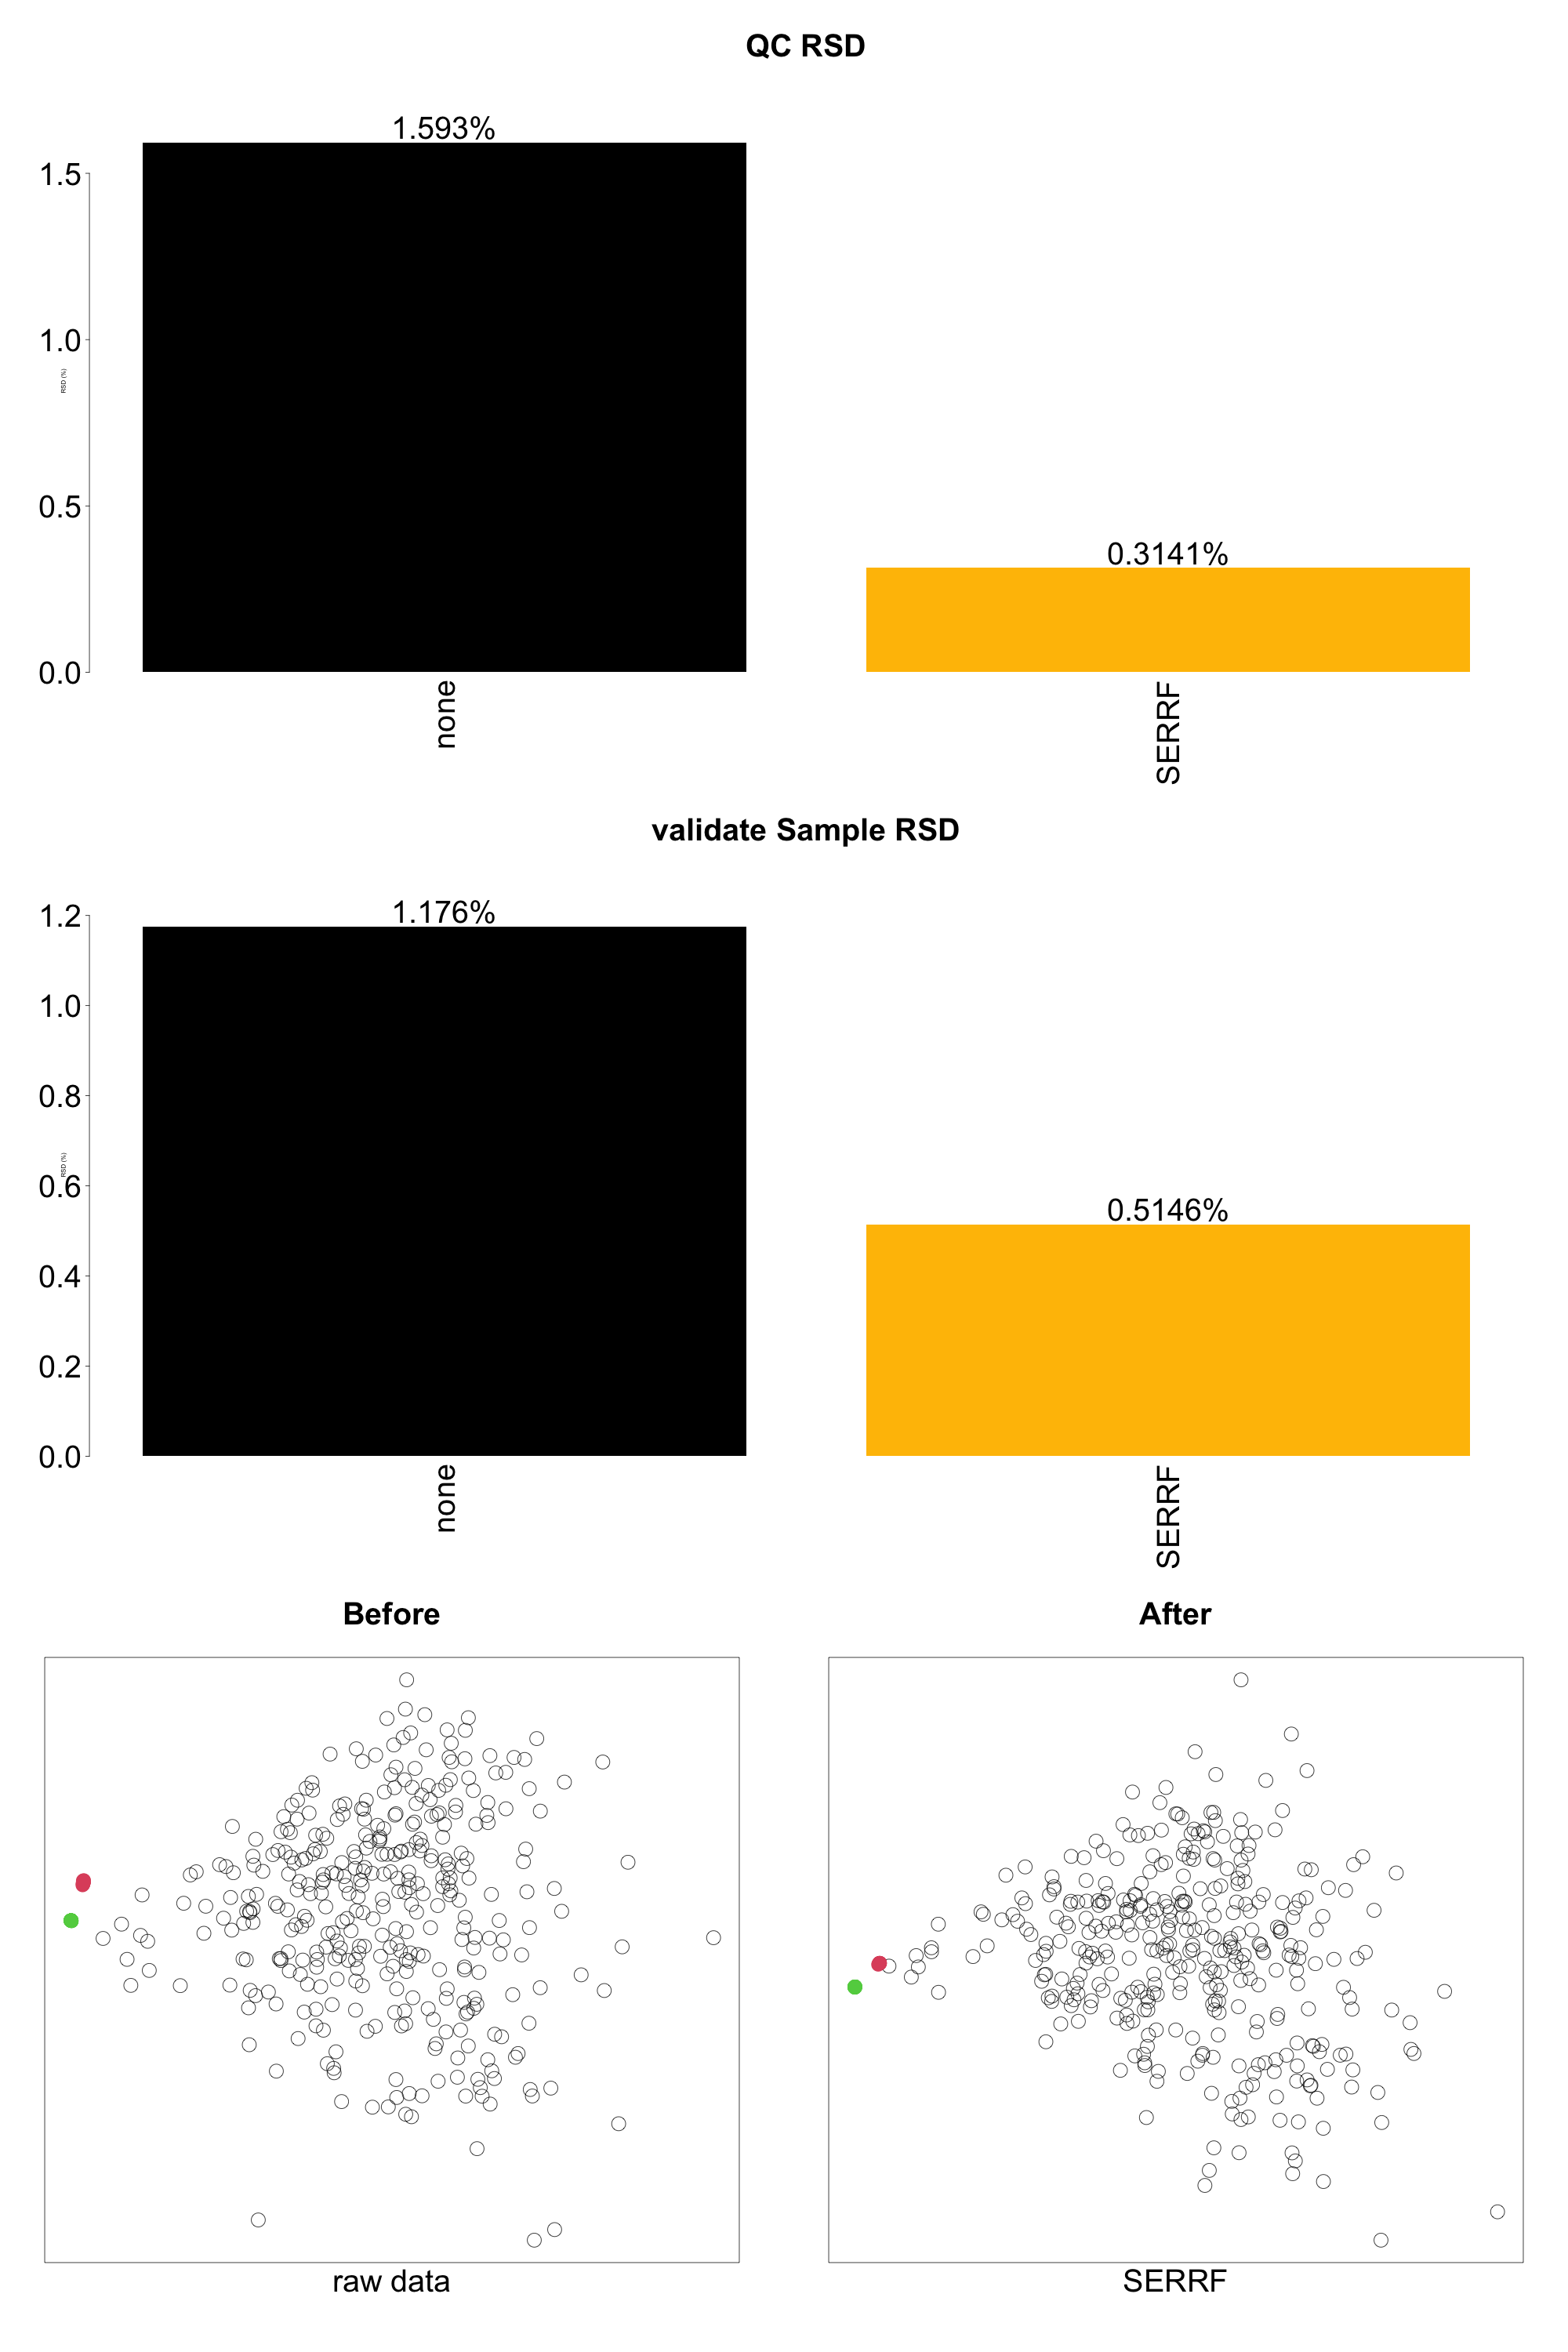
\includegraphics[width=\linewidth]{fig/supp/SuppFig_2B_RSD_PCA_Lowinput.png}
    \caption{Low‐Input.}
    \label{fig:S2B}
  \end{subfigure}

  \caption{
    SERRF-normalized quality metrics across injections.  
    (\textbf{A}) Control samples: per‐feature RSD distributions (boxplot) and PCA of QC vs.\ samples.  
    (\textbf{B}) Low‐Input samples: same metrics after SERRF correction.  
    Both panels demonstrate tight RSDs (most features<15 %) and clear separation of QC from biological samples in PC1/PC2.
  }
  \label{fig:S2}
\end{figure}







%========================================================
%  Supplementary Figure S3 - Lipid species/class count   (panels A, B, and C)
%========================================================
\begin{figure}[htp]
  \centering

  % ---------- row 1 ----------
  \begin{subfigure}[t]{0.48\textwidth}
    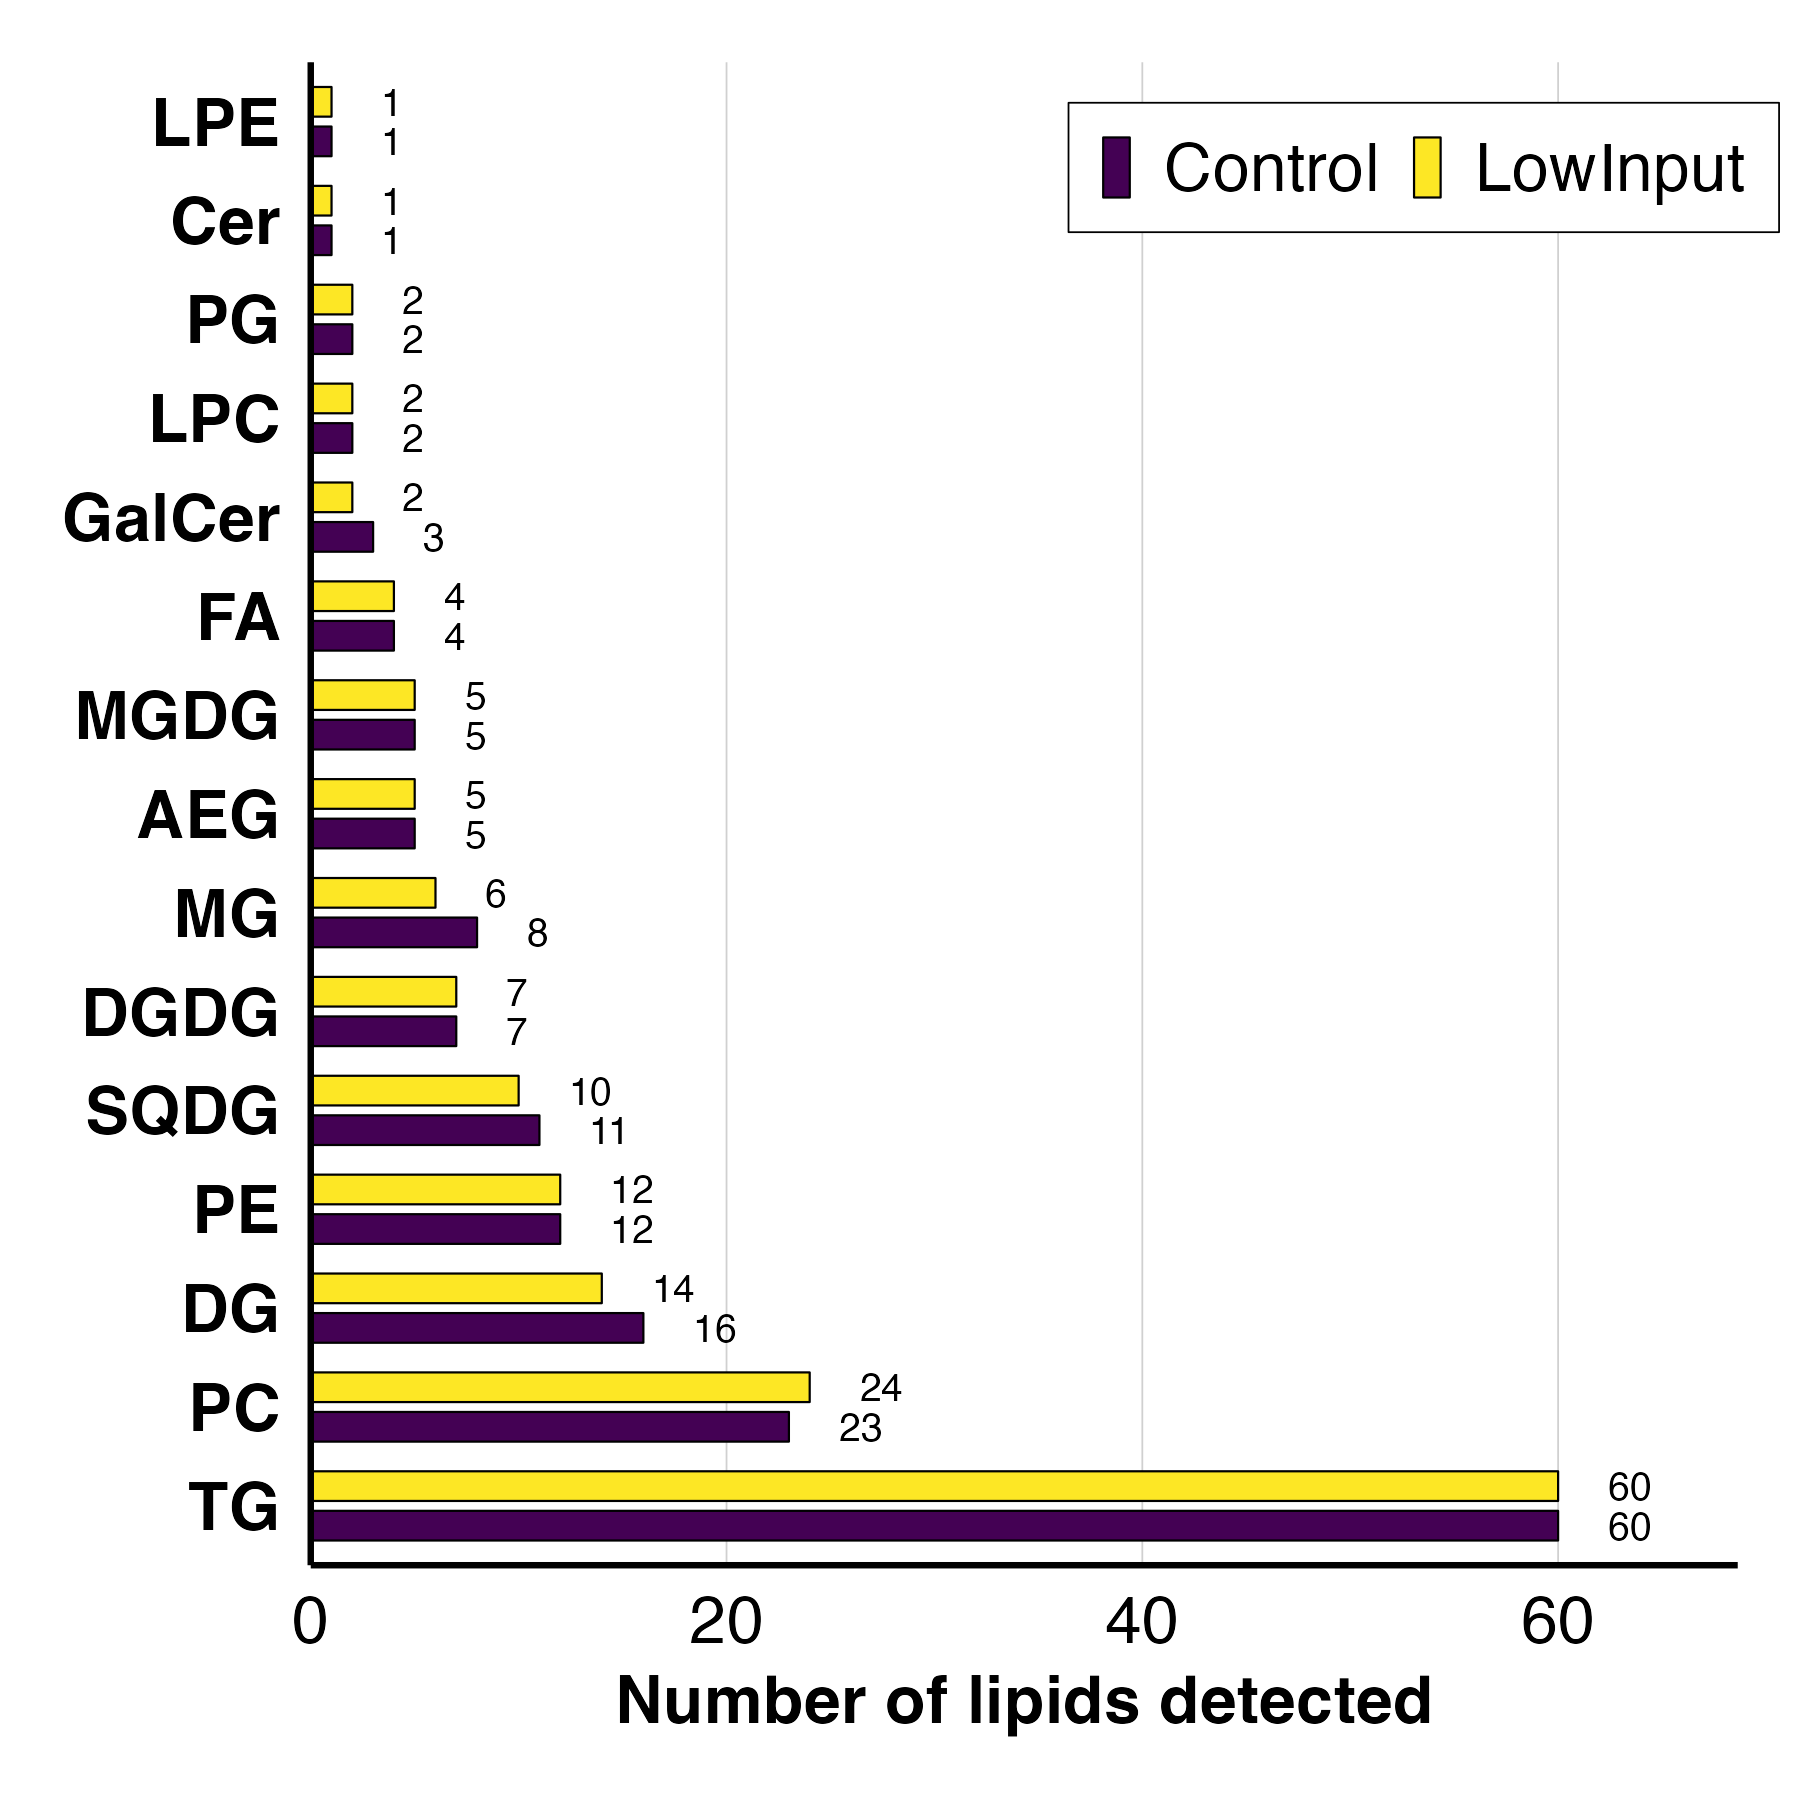
\includegraphics[width=\linewidth]{fig/supp/SuppFig_3A_Lipid_Counts}
    \caption{Number of lipid \textit{species}.}
    \label{fig:S3A}
  \end{subfigure}\hfill
  \begin{subfigure}[t]{0.48\textwidth}
    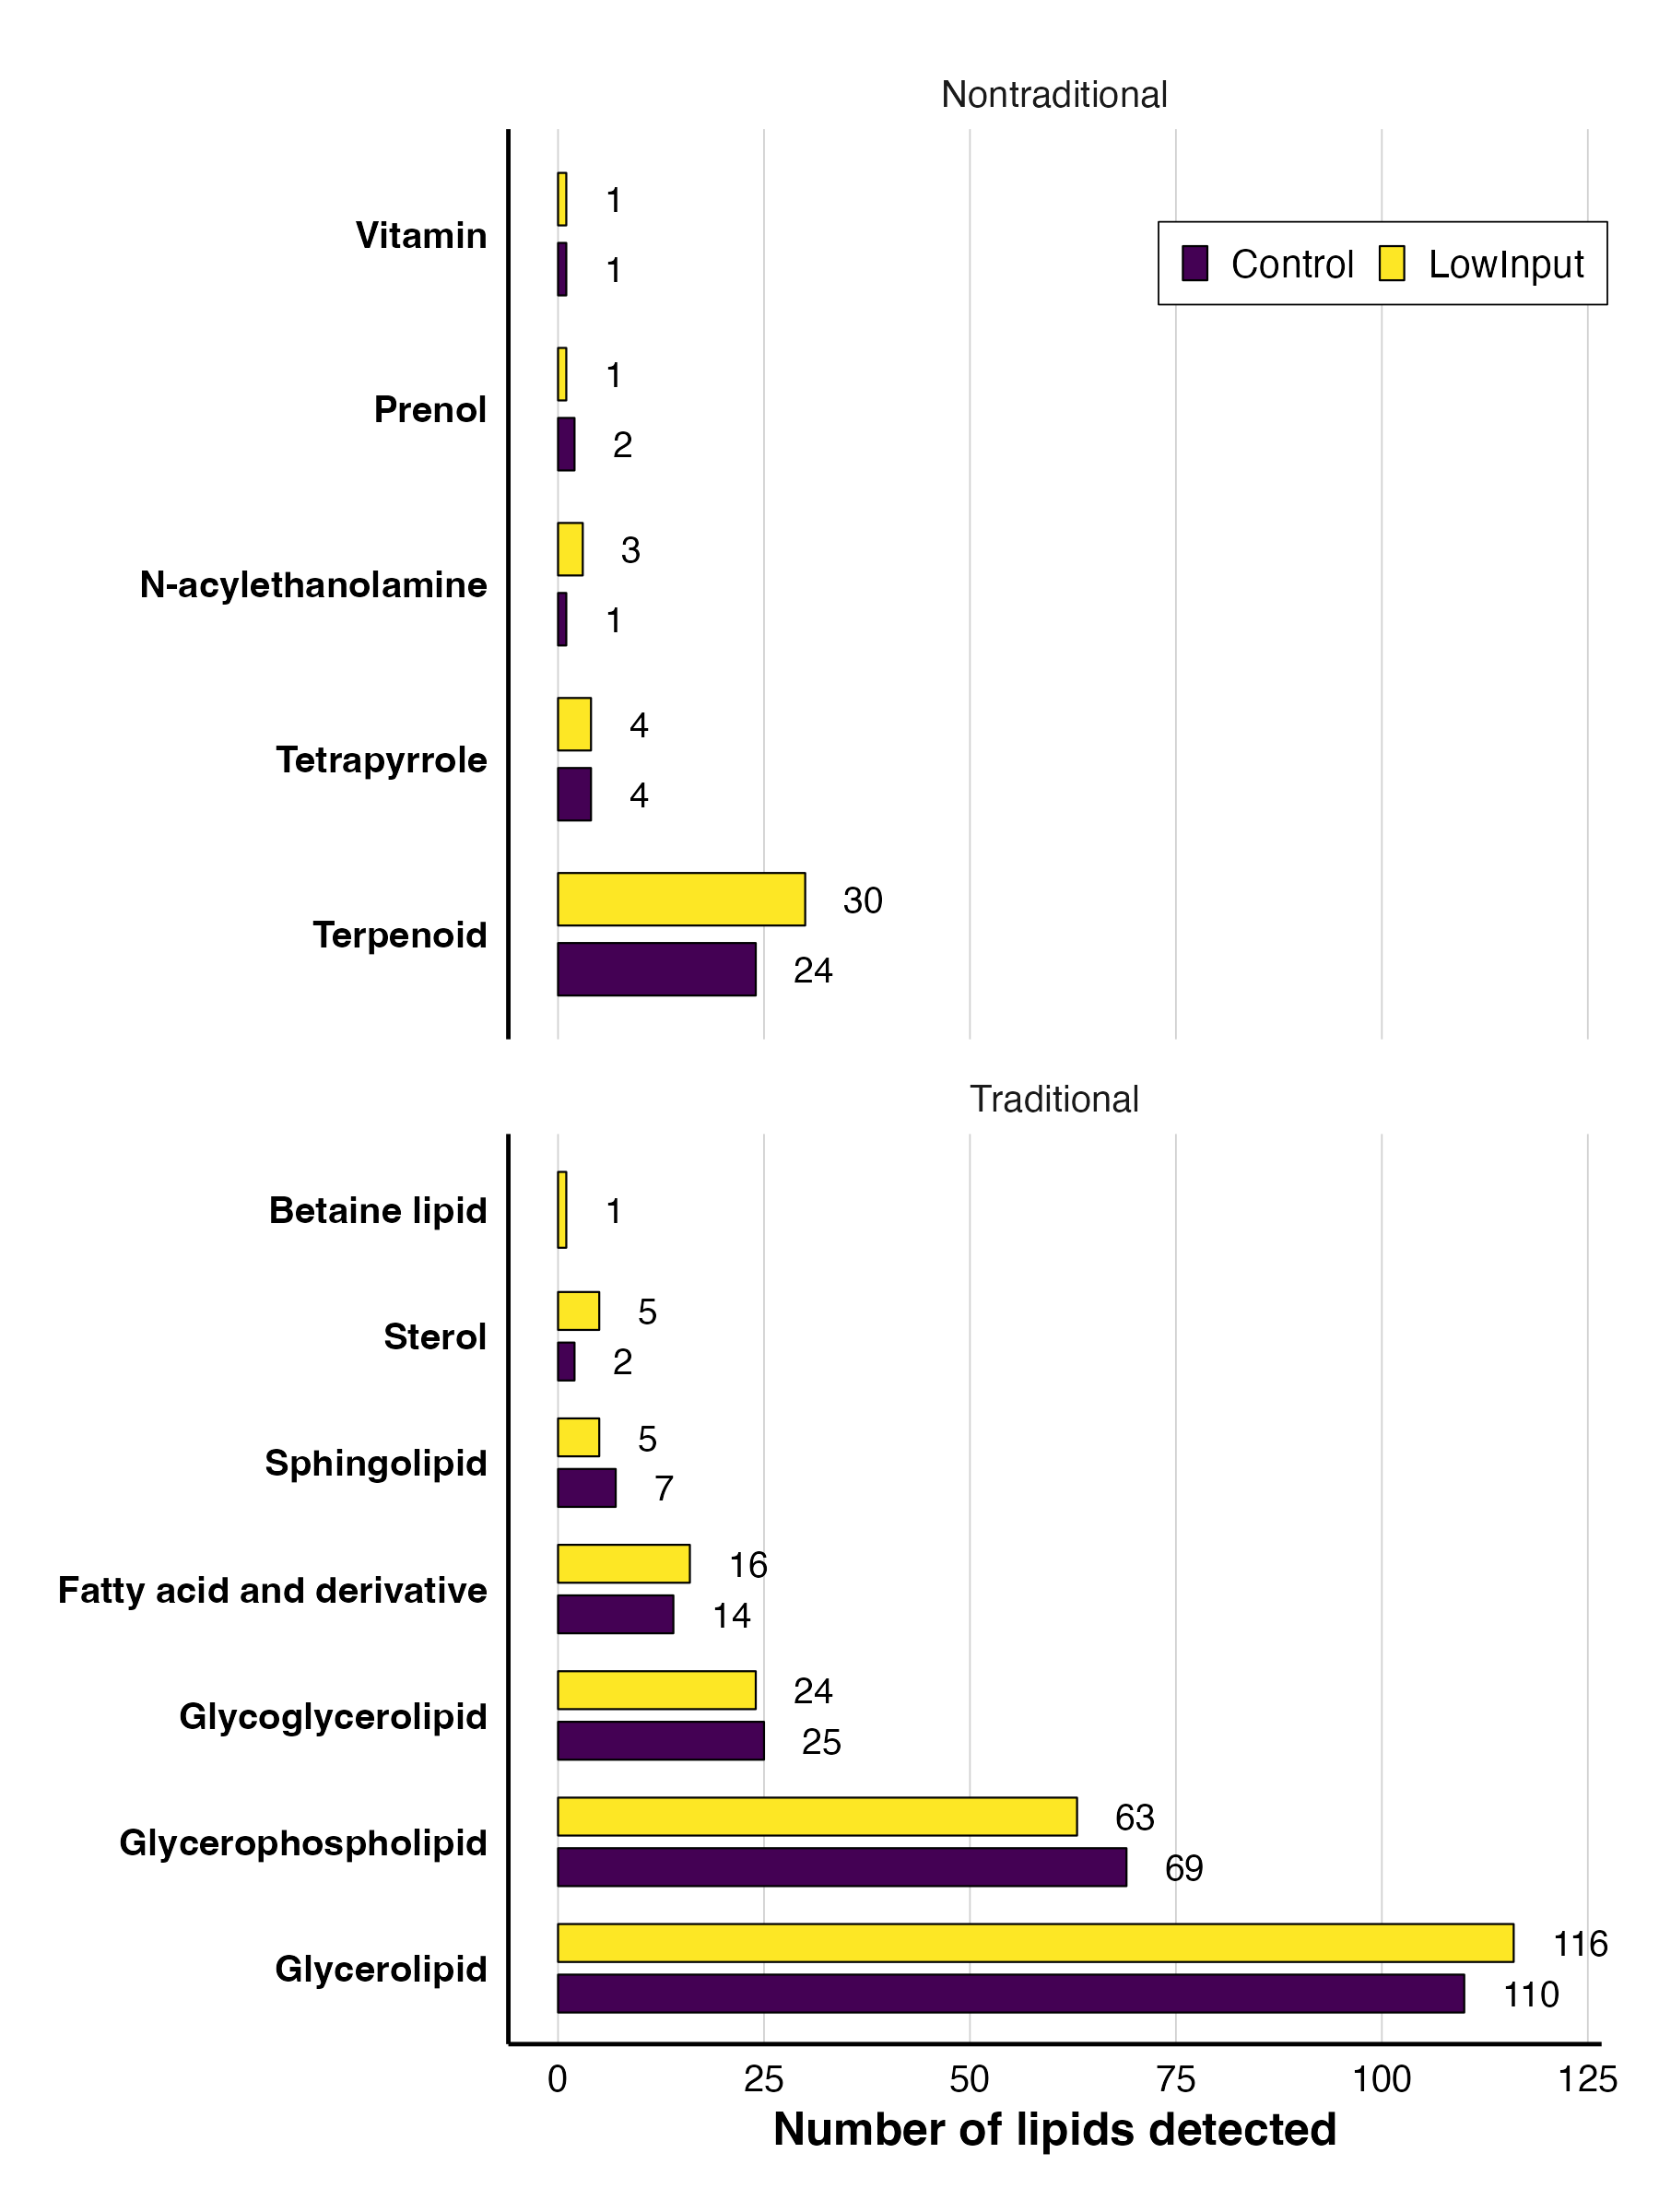
\includegraphics[width=\linewidth]{fig/supp/SuppFig_3B_Lipid_Class_Counts}
    \caption{Number of lipid \textit{classes}.}
    \label{fig:S3B}
  \end{subfigure}

  \vspace{1em}

  % ---------- row 2 (centred) ----------
  \begin{subfigure}[t]{0.55\textwidth}
    \centering
    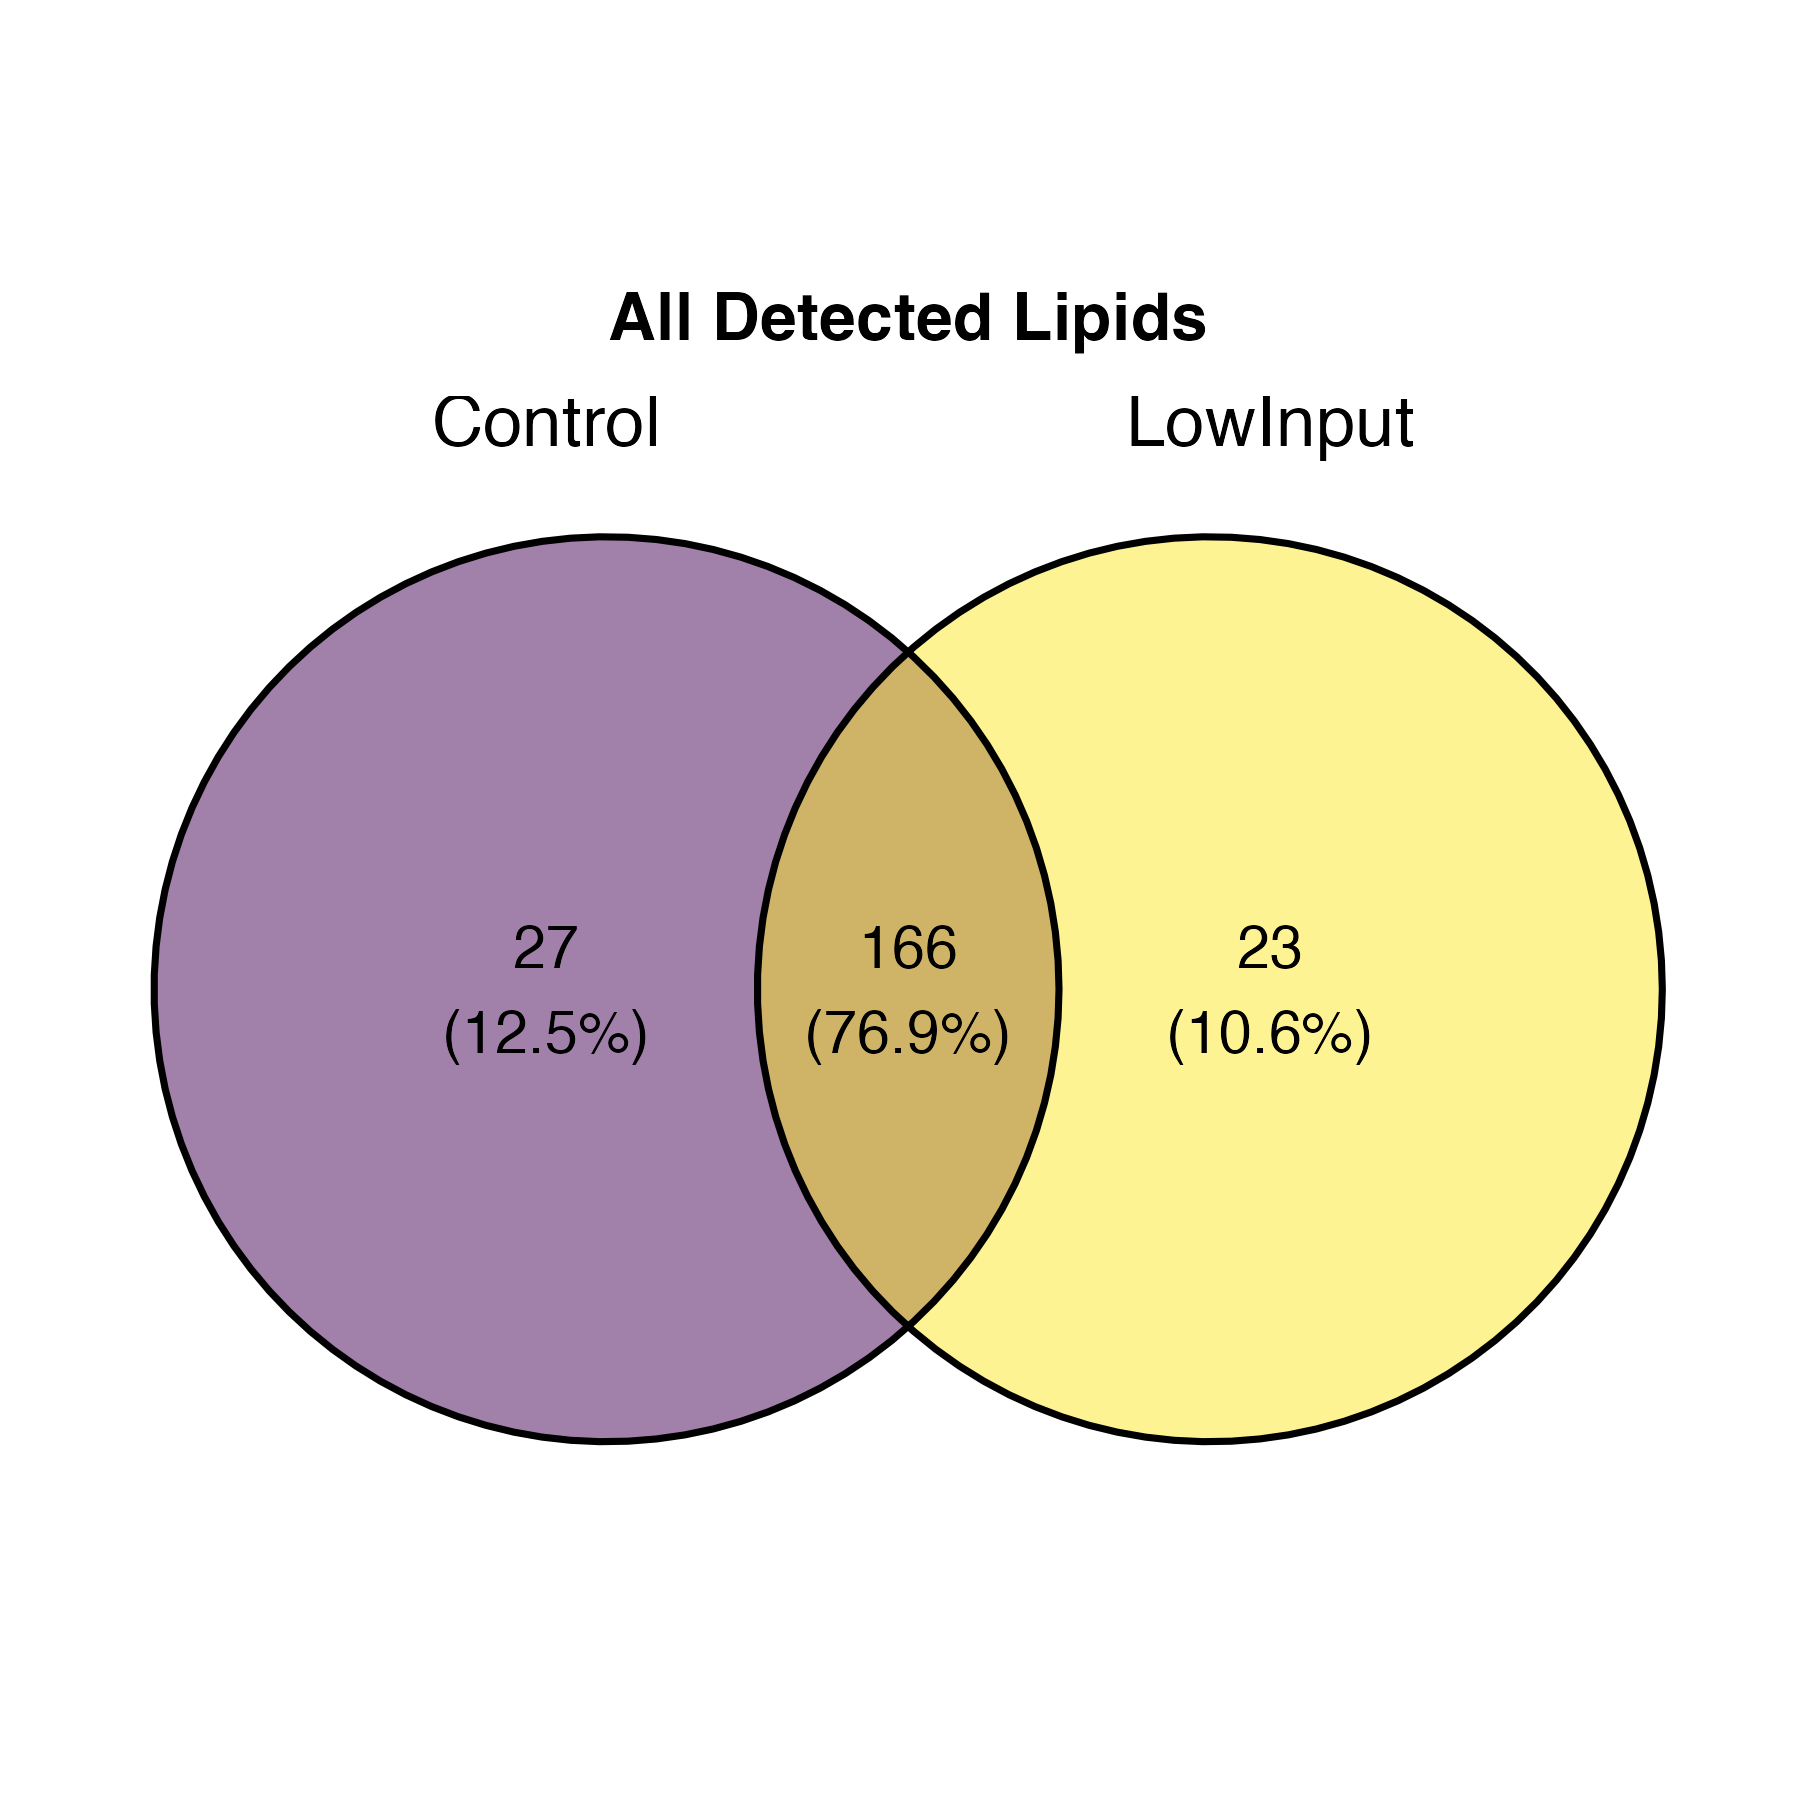
\includegraphics[width=\linewidth]{fig/supp/SuppFig_3C_Lipid_Overlap_Venn}
    \caption{Shared and unique lipid species.}
    \label{fig:S3C}
  \end{subfigure}

  \caption{Overview of lipid coverage in Control and Low-Input samples.}
  \label{fig:S3}
\end{figure}


%========================================================
%  Supplementary Figure S4 - Lipid ratio contrasts under low-P
%========================================================
\begin{figure}[htp]
  \centering
  % Adjust width fraction as needed (e.g., 0.8\textwidth or \textwidth)
  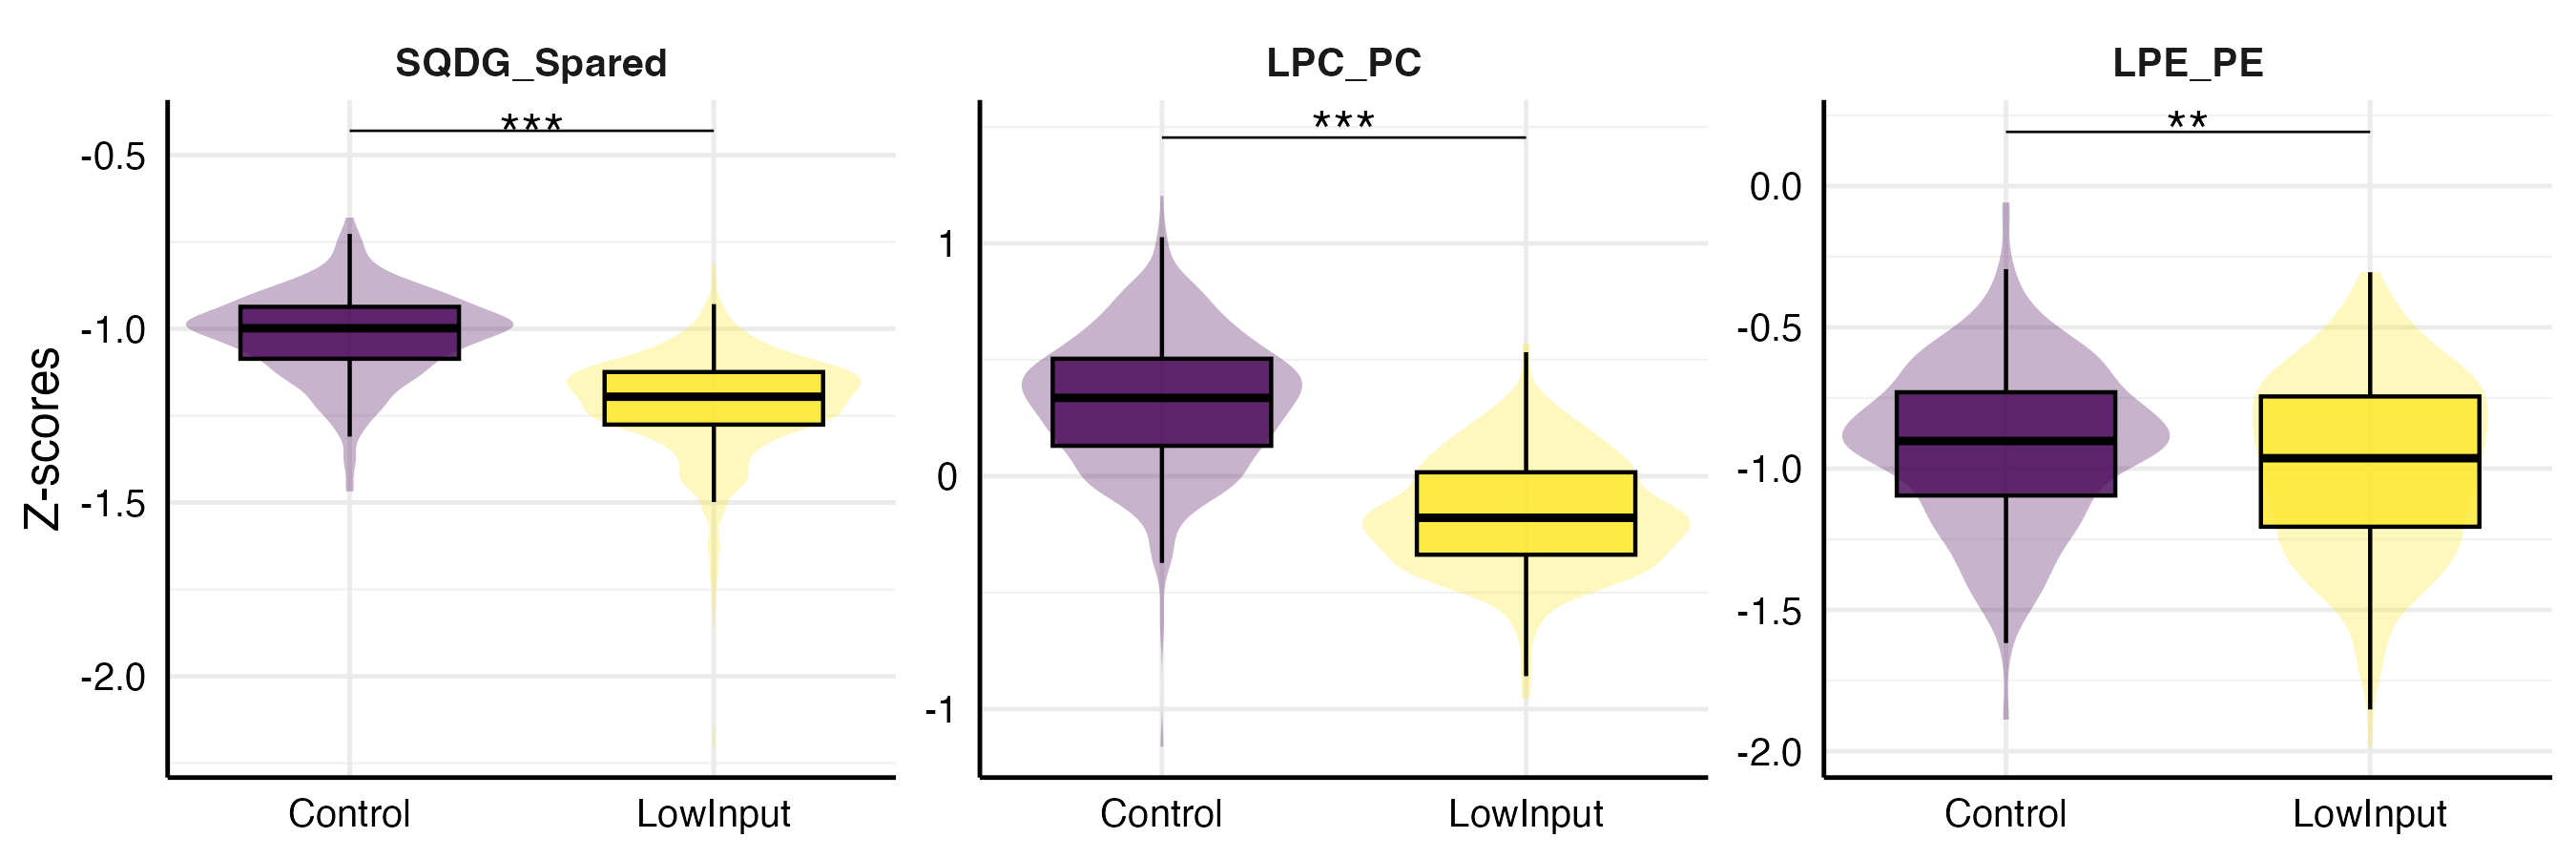
\includegraphics[width=0.8\textwidth]{fig/supp/SuppFig_4_lipid_ratio_linear_lowP.png}
  \caption{ΔZ-score contrasts for lipid ratio metrics under phosphorus deprivation (low-P). 
    The panel shows violin+boxplots for metrics such as SQDG\_Spared, LPC/PC, and LPE/PE under Control versus LowInput conditions. 
    Stars denote significance levels (***: $p<0.001$, **: $p<0.01$, *: $p<0.05$) from appropriate statistical tests. 
    A negative ΔZ in SQDG\_Spared indicates sulfolipid is not upregulated relative to galactolipids and PG; 
    LPC/PC is not significantly changed, whereas LPE/PE and composite Lyso\_activity shift toward values consistent with selective PE deacylation.}
  \label{fig:S4_lipid_ratio_lowP}
\end{figure}

%========================================================
%  Supplementary Figure S5 - TIC Proportions for LPC and LPE
%========================================================
\begin{figure}[htp]
  \centering
  % Adjust width fraction as appropriate, e.g., 0.6\textwidth or \textwidth
  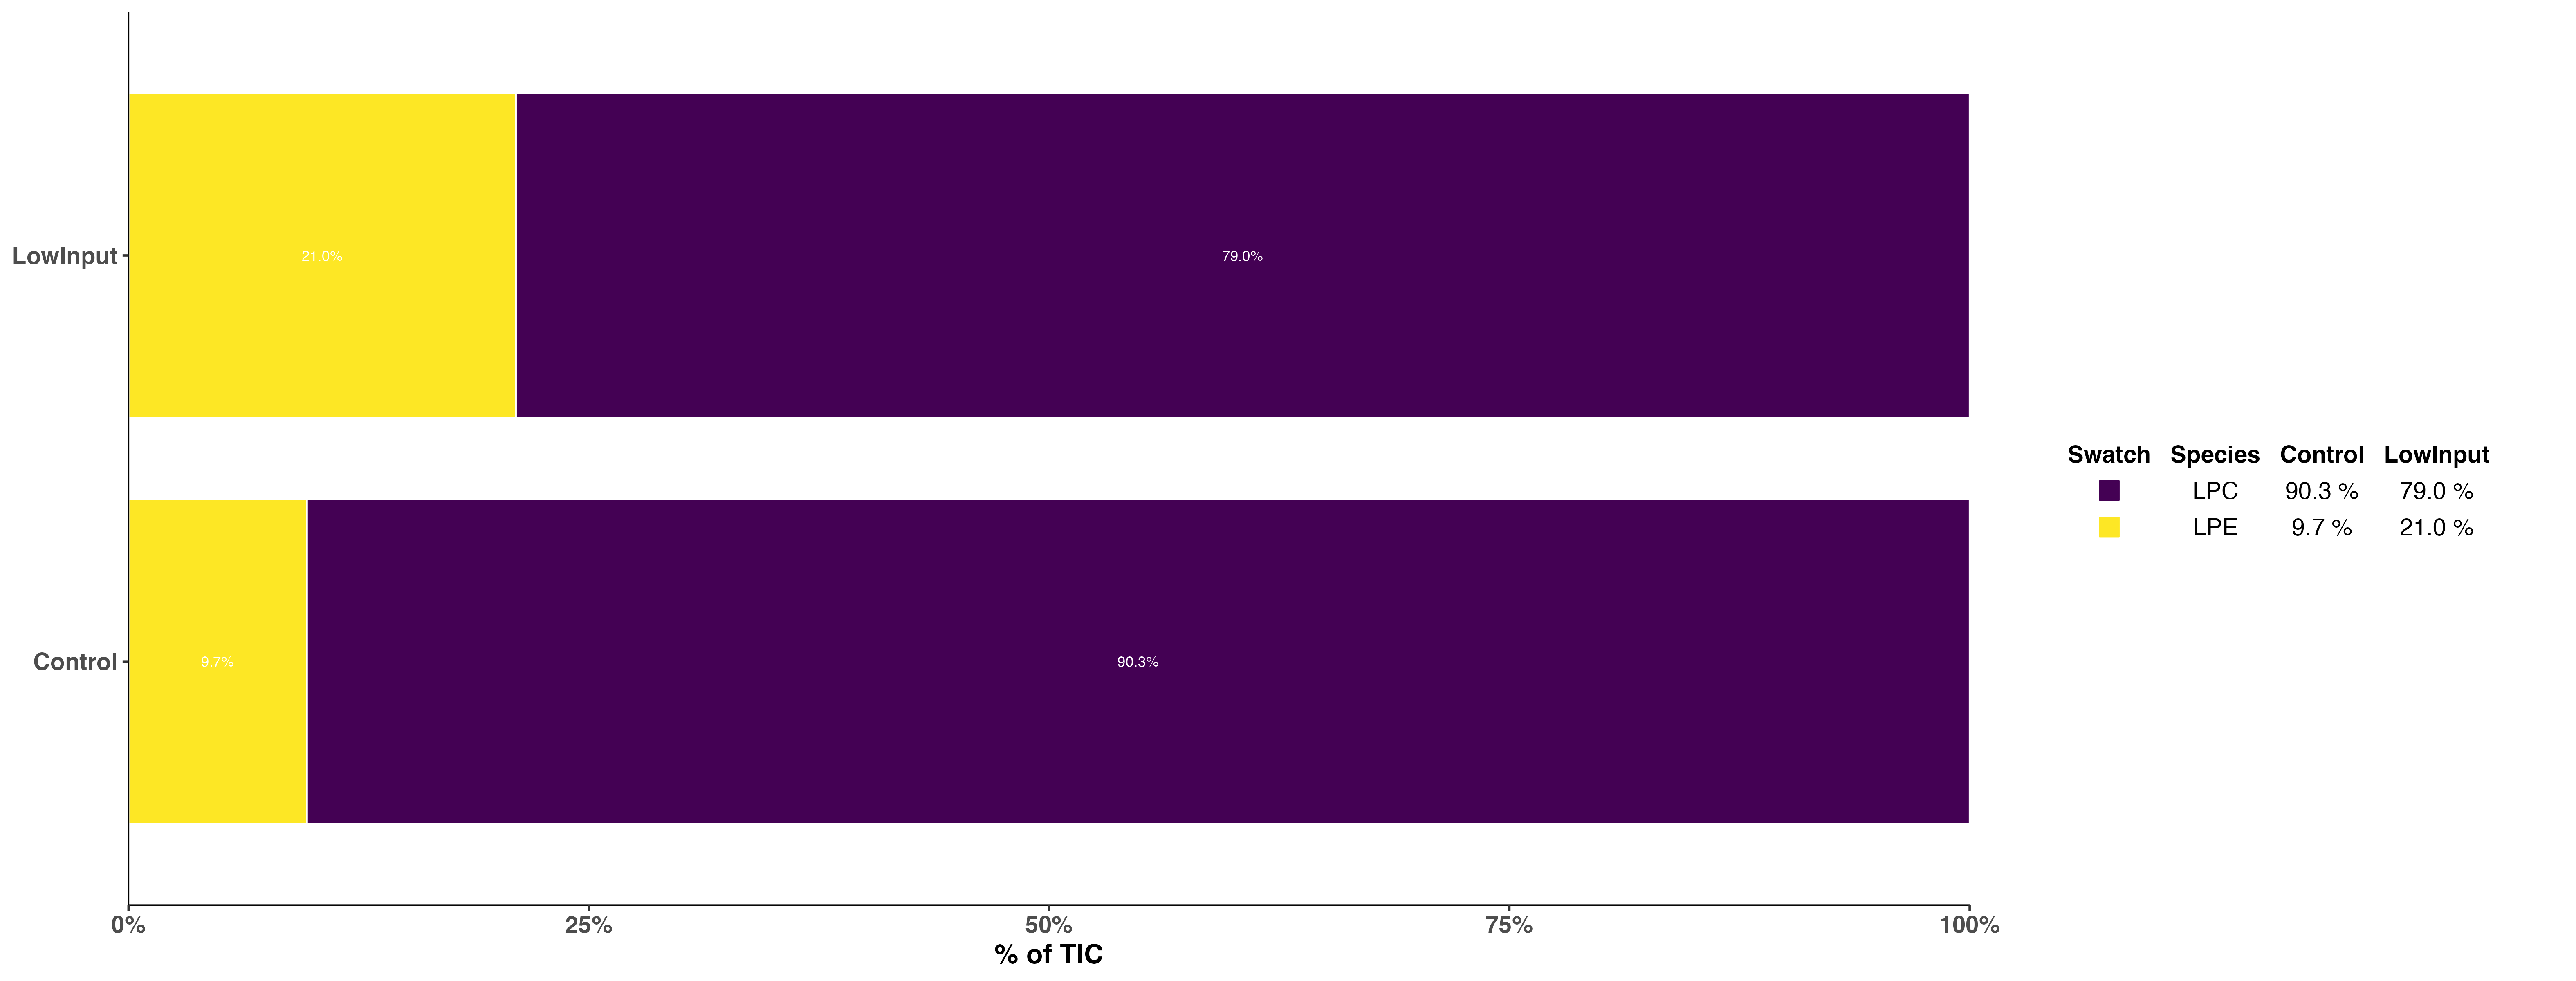
\includegraphics[width=0.7\textwidth]{fig/supp/SuppFig_5_TIC_LPC_LPE.png}
  \caption{Total ion current (TIC) proportions of lysophosphatidylcholine (LPC) and lysophosphatidylethanolamine (LPE) under Control and Low-P conditions. The plot displays relative TIC share of LPC versus LPE; stars denote significance levels (e.g., *: $p<0.05$, **: $p<0.01$) from appropriate tests. An increase in the LPE fraction and corresponding decrease in LPC under low-P suggests selective deacylation of PE for P salvage, while PC-derived LPC remains relatively stable.}
  \label{fig:S5_TIC_LPC_LPE}
\end{figure}



\end{document}


